\section*{Question 8}
\fakesection{8}

This exercise extends Question 7 to investigate how stability is impacted by increasing the order of the Butterworth filter. To this end, 5th, 6th, 7th, and 8th-order filters are investigated. For brevity, the outcomes are discussed first, and the supporting figures are provided over the following pages.

\begin{enumerate}[label=\alph*)]

    \item As filter order increases, the arc of poles in the right half-plane approaches the unit circle. The number of poles is equal to the order of the filter, so as the order increases, more poles are packed into the right half-plane. Furthermore, as the order increases, greater decimal precision is required for the root-finding arithmetic. As the required precision exceeds the available precision, the locations of the poles become increasingly divergent and eventually move outside the unit circle, at which point the filter becomes unstable.

    A very similar observation can be made of the zeros. In theory, the zeros of a Butterworth low pass filter should all coincide at -1. However, we observe that due to insufficient numerical precision, the zeros become increasingly spread out around -1. This is most evident for the quantized coefficients, but is non-negligible for the 8th-order filter even with full float precision. Unlike the poles, however, this does not induce instability.

    \item Using a binary search trial and error technique, the maximum stable filter orders were determined both before and after quantization. These were orders 31 and 10, respectively.

\end{enumerate}

The supporting figures are presented over the following eight pages, one page for each different filter order. In order, these are orders: 5, 6, 7, 8, 10, 11, 31, and 32. Each page presents:
\begin{itemize}
    \item the frequency gain and phase response;
    \item the pole-zero plot; and
    \item the experimental frequency and time responses.
\end{itemize}
For filter orders 5 through 8, plots are provided for both before and after quantization. For filter orders 10 and 11, plots are provided for after quantization only. For filter orders 31 and 32, plots are provided for before quantization only.

\newpage
{\Large\textbf{Filter Order: 5 (Unquantized and Quantized)}}
\vfill

\begin{figure}[ht]
    \centering
    \begin{subfigure}[b]{0.56\textwidth}
        \centering
        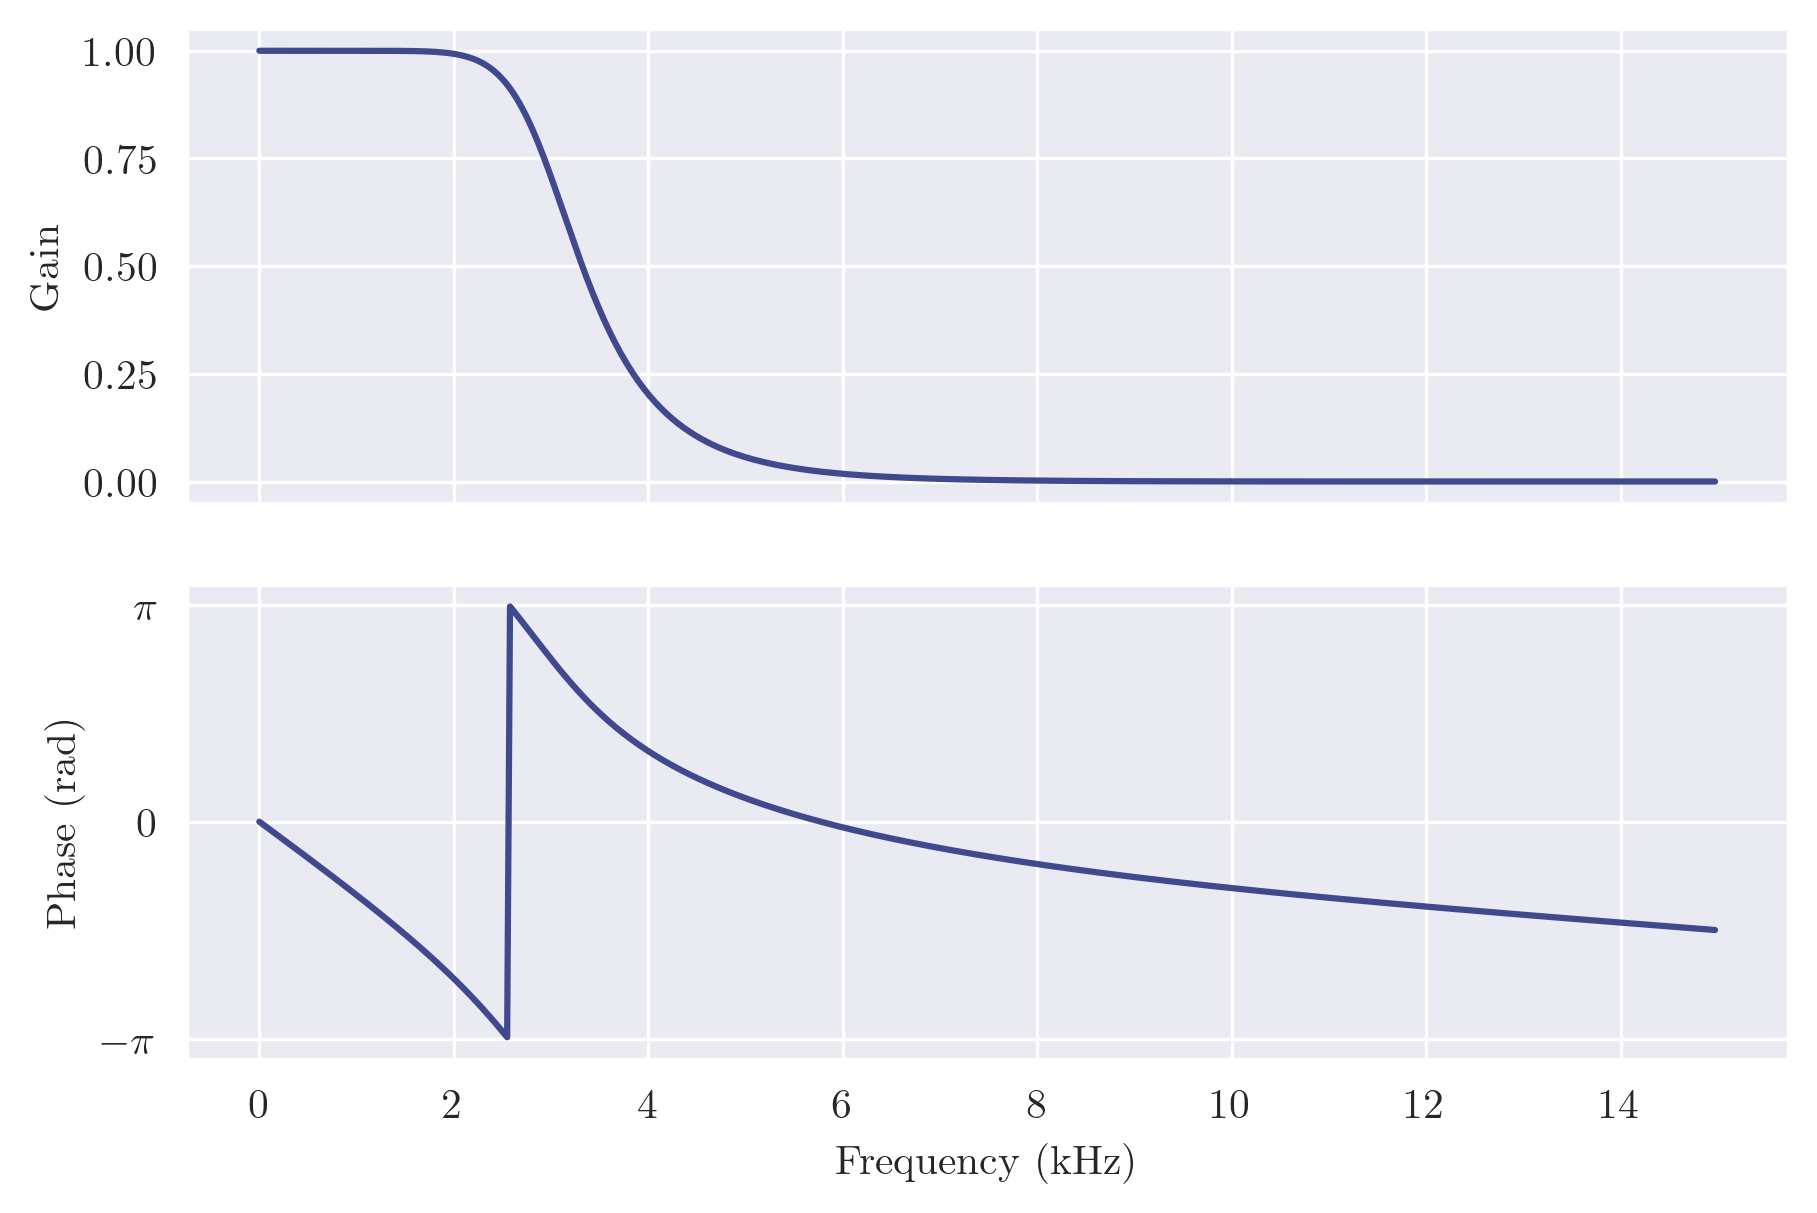
\includegraphics[width=\textwidth]{images/q8_5th_freqz.png}
    \end{subfigure}
    \hfill
    \begin{subfigure}[b]{0.43\textwidth}
        \centering
        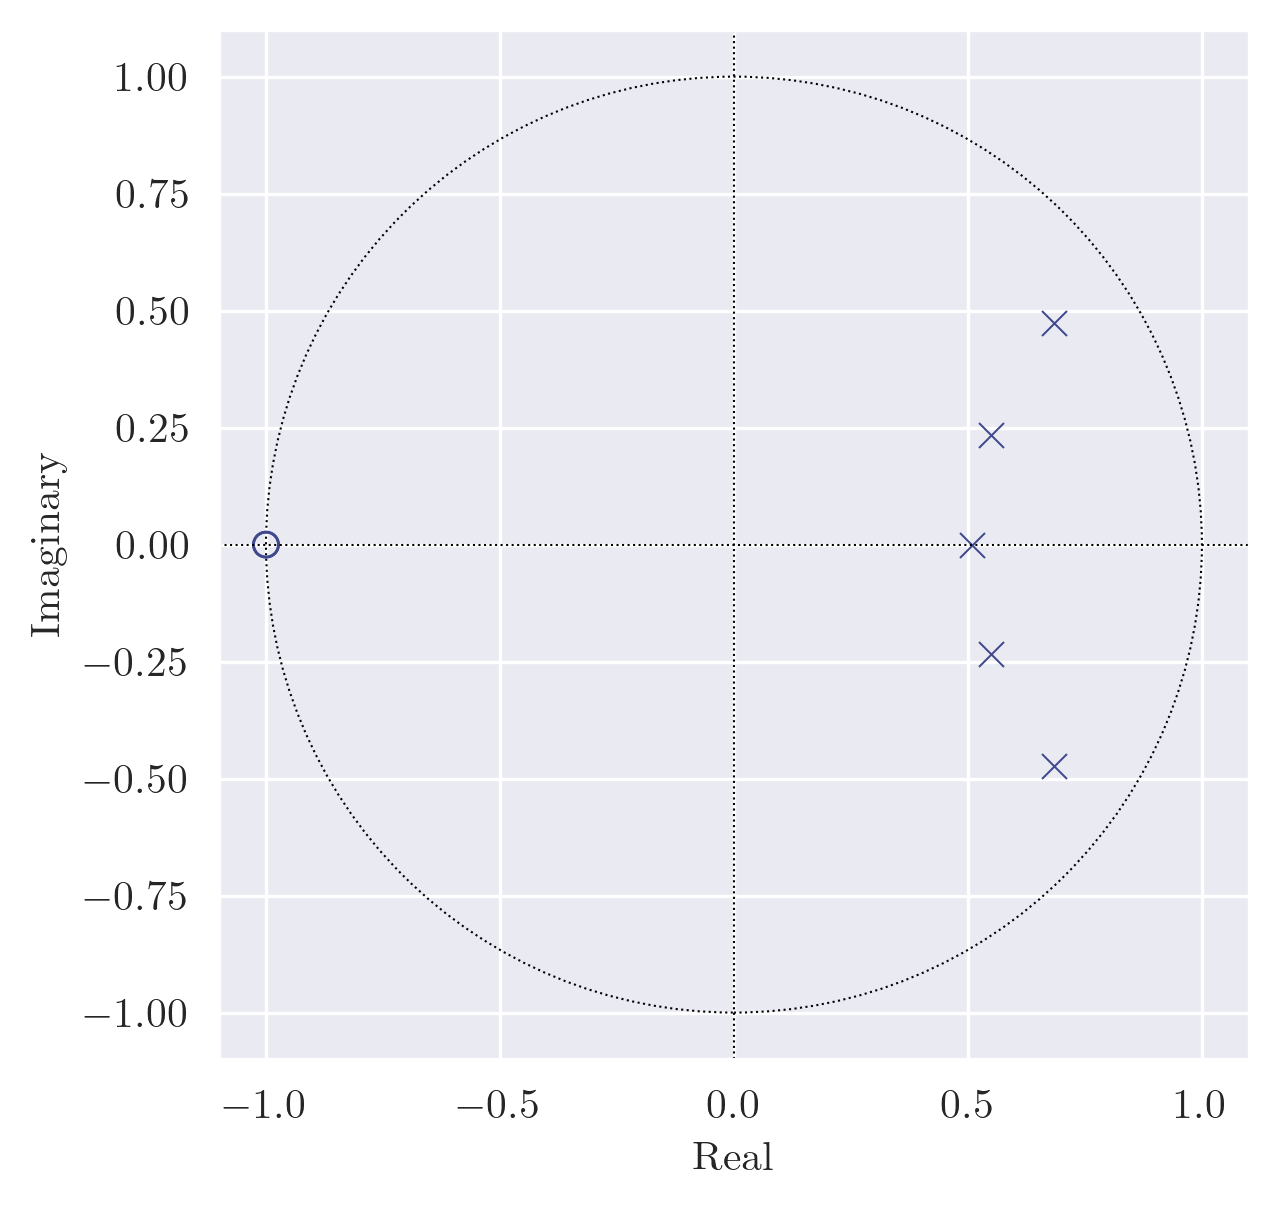
\includegraphics[width=\textwidth]{images/q8_5th_zp.png}
    \end{subfigure}
    \caption{Frequency response and pole-zero plot of 5th-order low pass Butterworth filter}
\end{figure}

\begin{figure}[!ht]
    \centering
    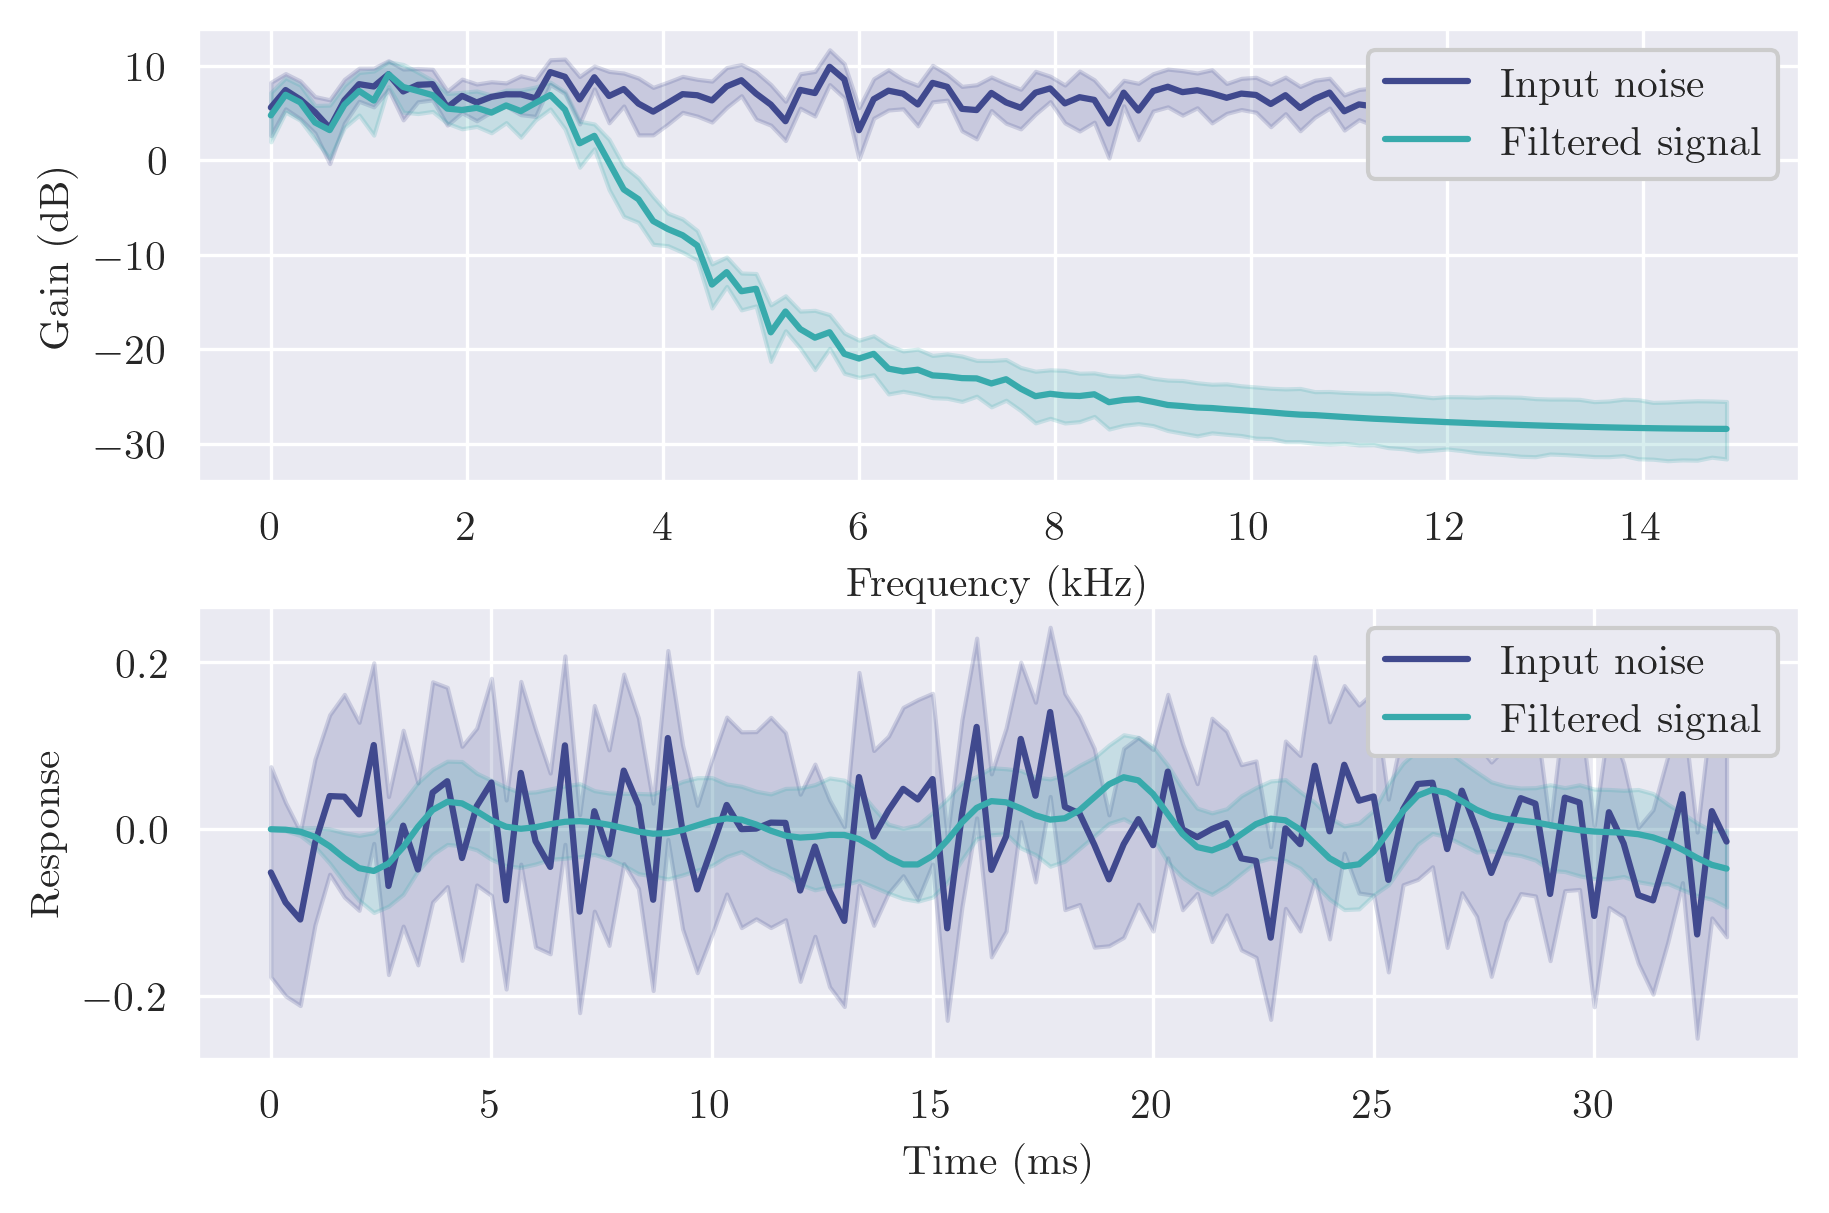
\includegraphics[width=0.99\textwidth]{images/q8_5th_stability.png}
    \caption{Original and (5th-order) filtered noise signals using unquantized coefficients}
\end{figure}

\begin{figure}[!ht]
    \centering
    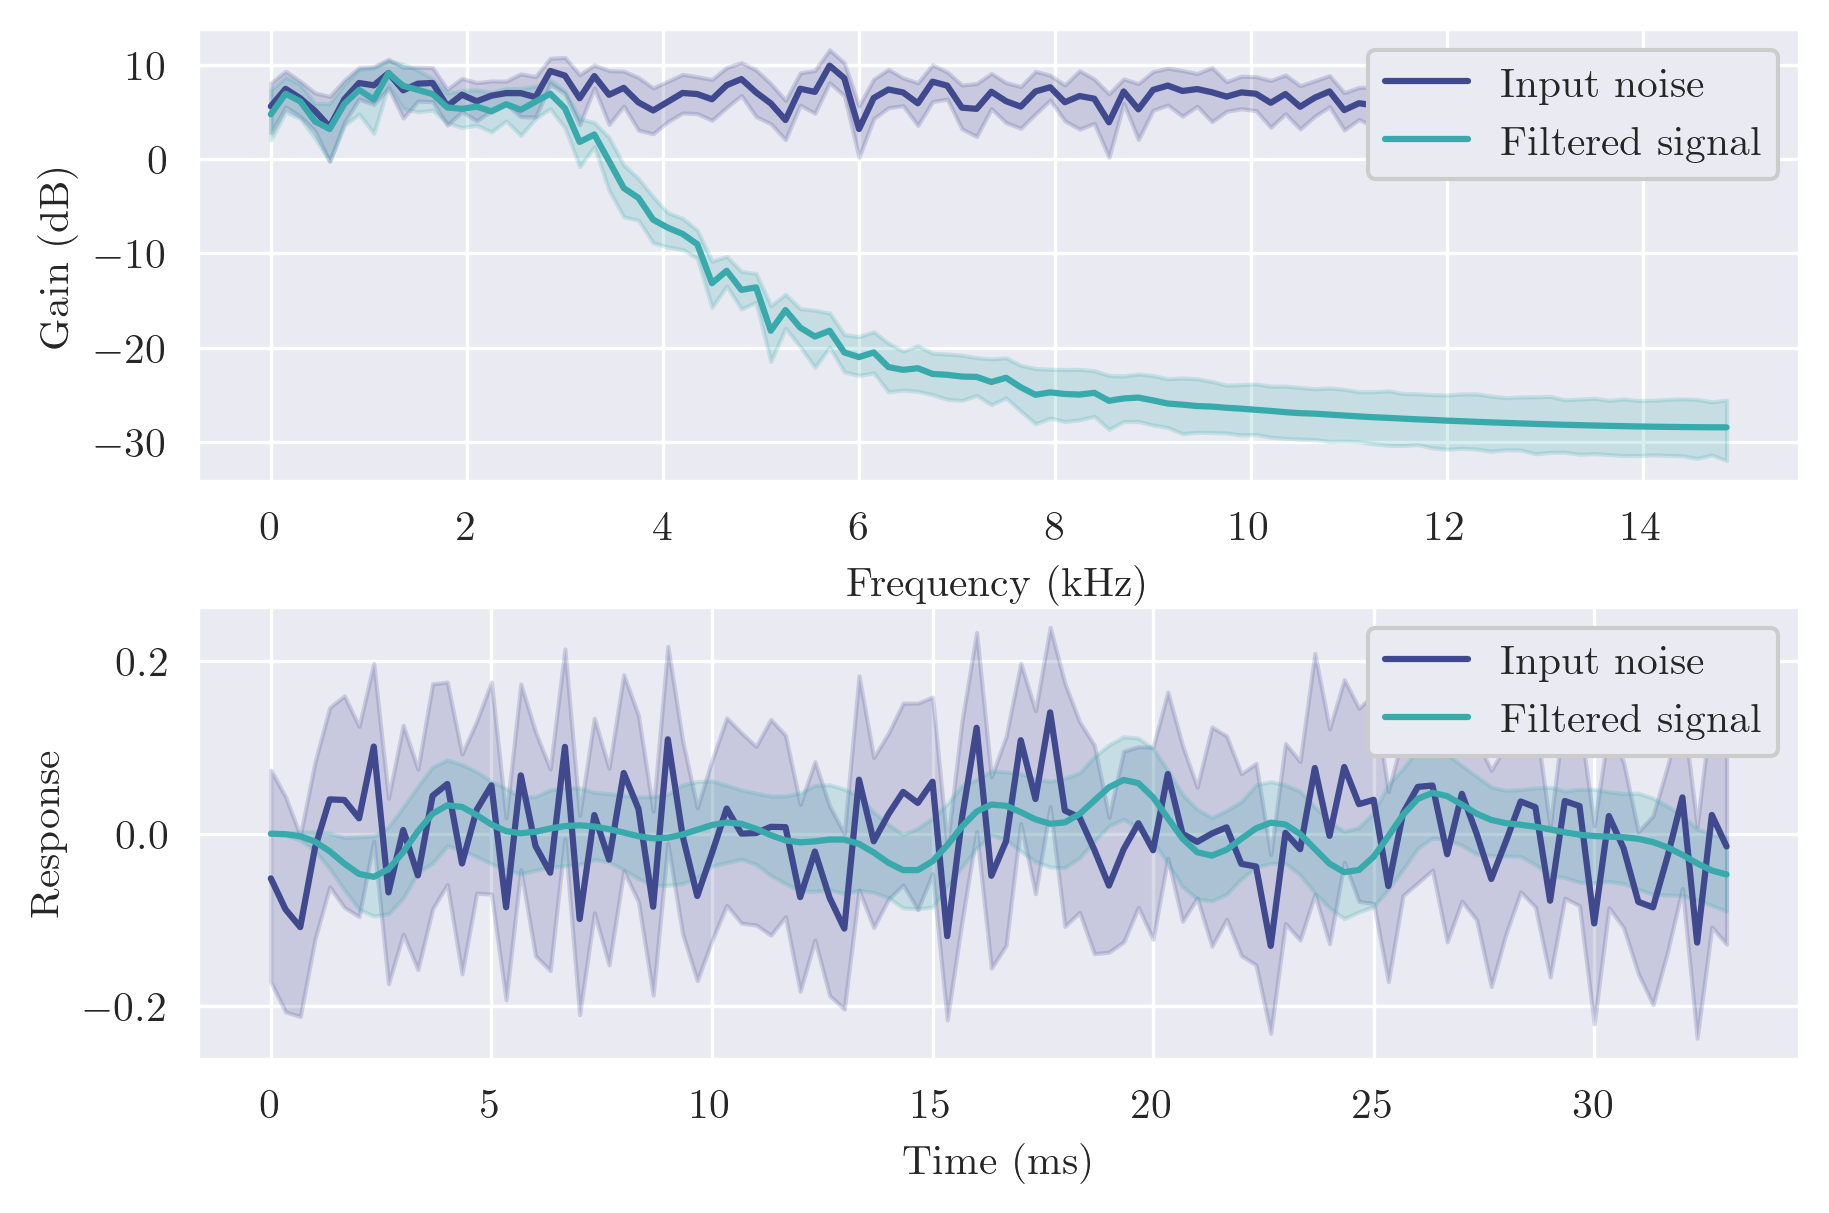
\includegraphics[width=0.99\textwidth]{images/q8_q5th_stability.png}
    \caption{Original and (5th-order) filtered noise signals using quantized coefficients}
\end{figure}

\newpage
{\Large\textbf{Filter Order: 6 (Unquantized and Quantized)}}
\vfill

\begin{figure}[ht]
    \centering
    \begin{subfigure}[b]{0.56\textwidth}
        \centering
        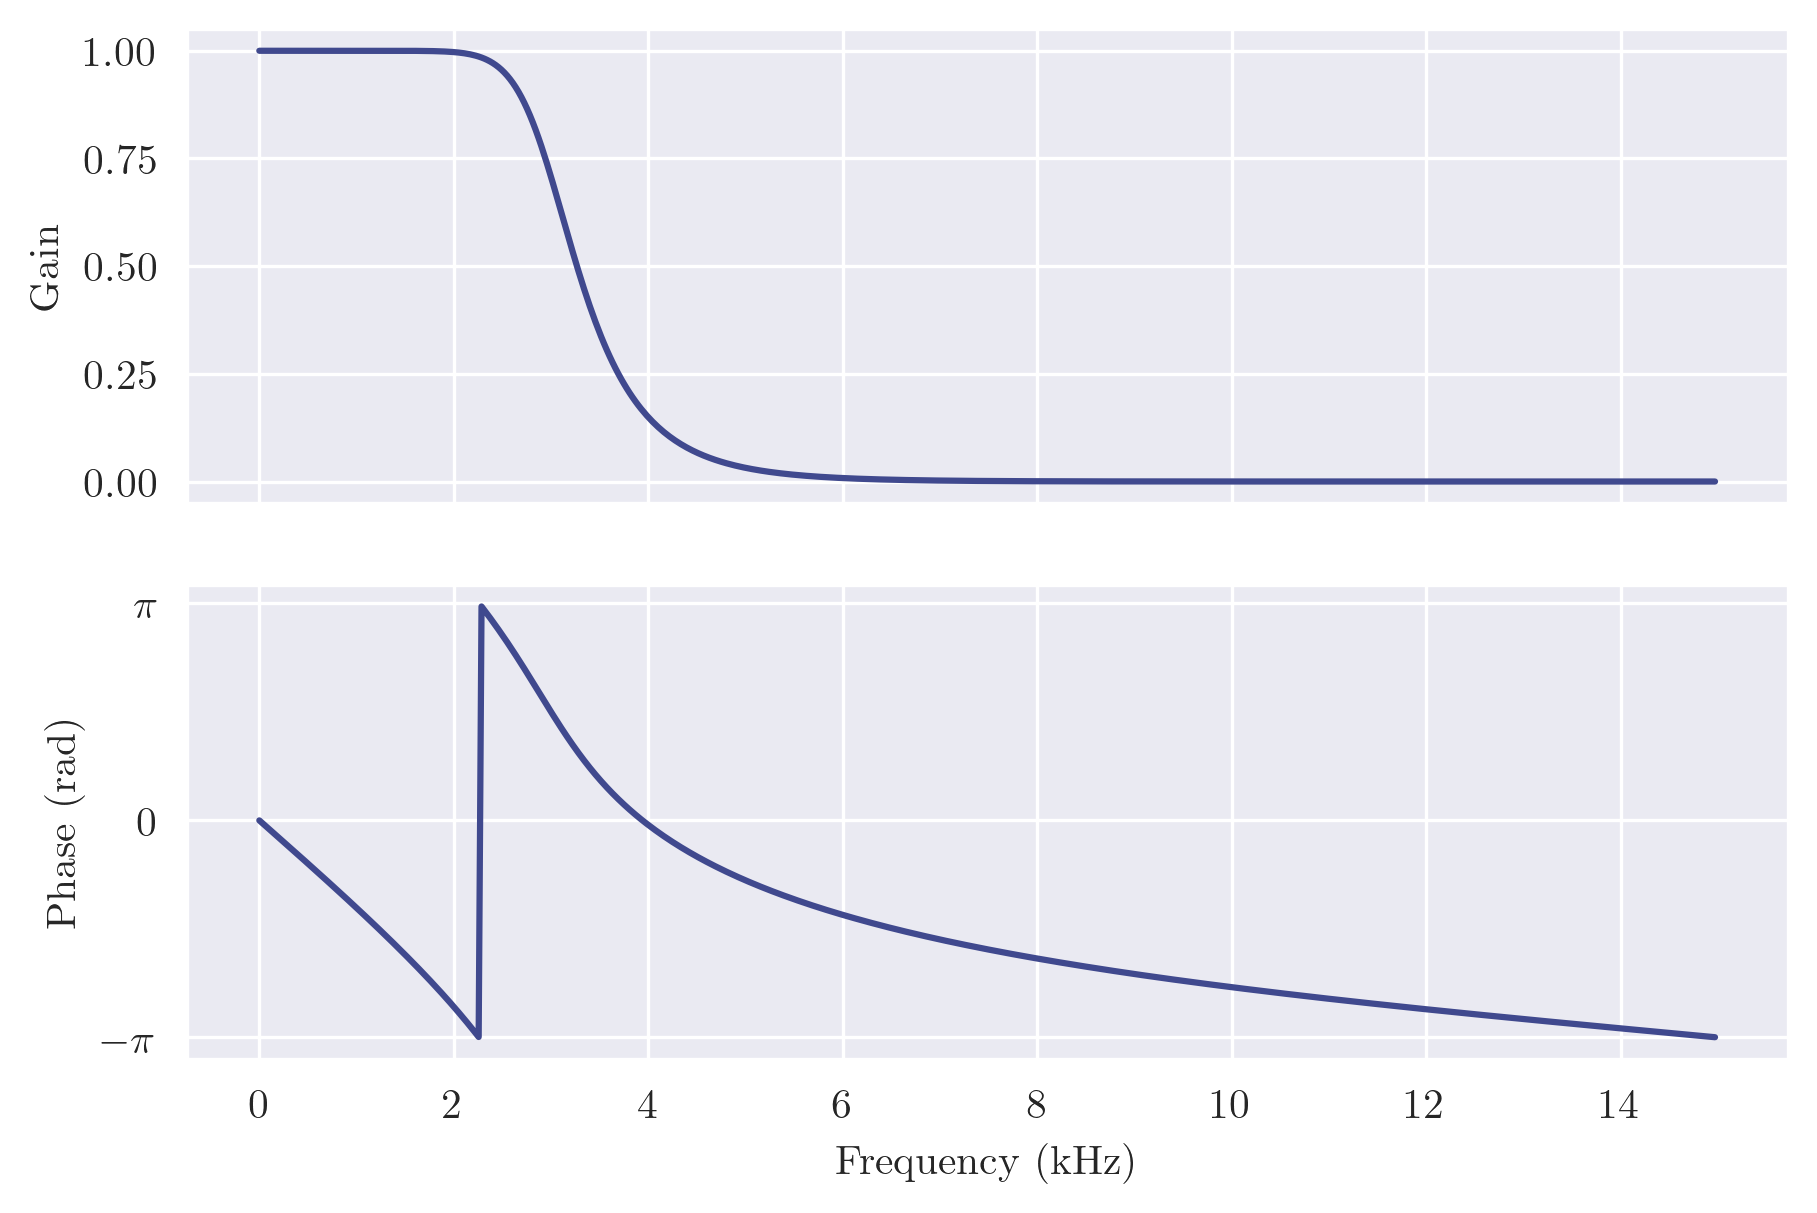
\includegraphics[width=\textwidth]{images/q8_6th_freqz.png}
    \end{subfigure}
    \hfill
    \begin{subfigure}[b]{0.43\textwidth}
        \centering
        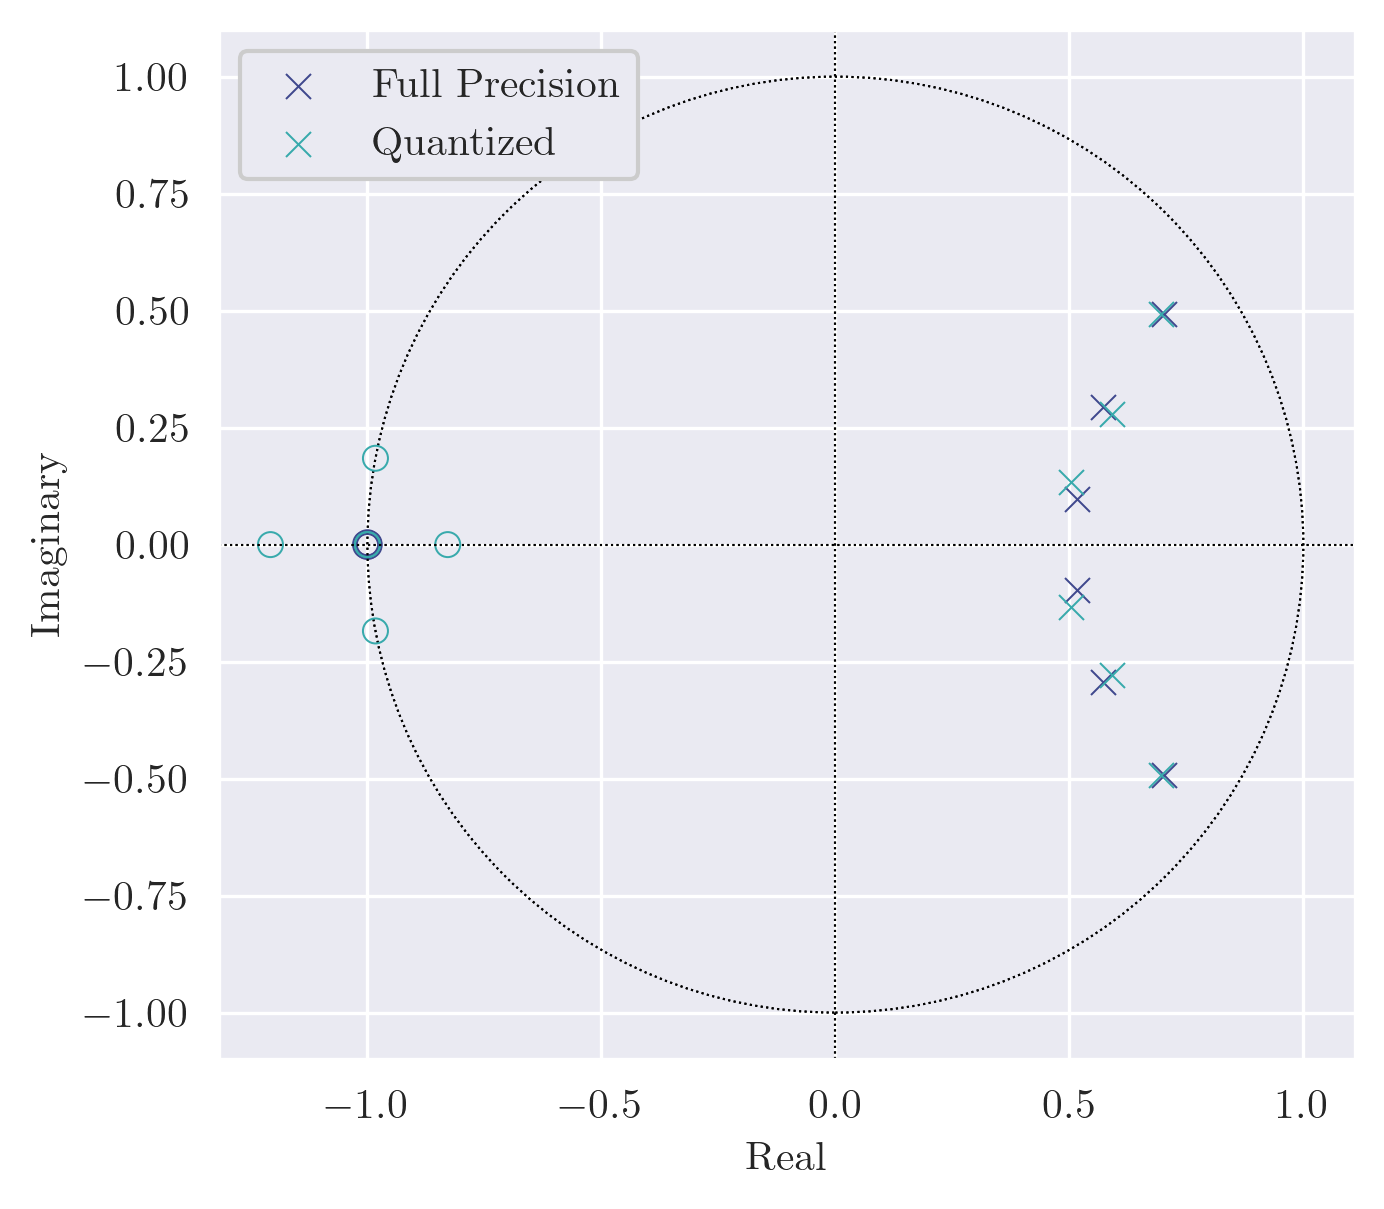
\includegraphics[width=\textwidth]{images/q8_6th_zp.png}
    \end{subfigure}
    \caption{Frequency response and pole-zero plot of 6th-order low pass Butterworth filter}
\end{figure}

\begin{figure}[!ht]
    \centering
    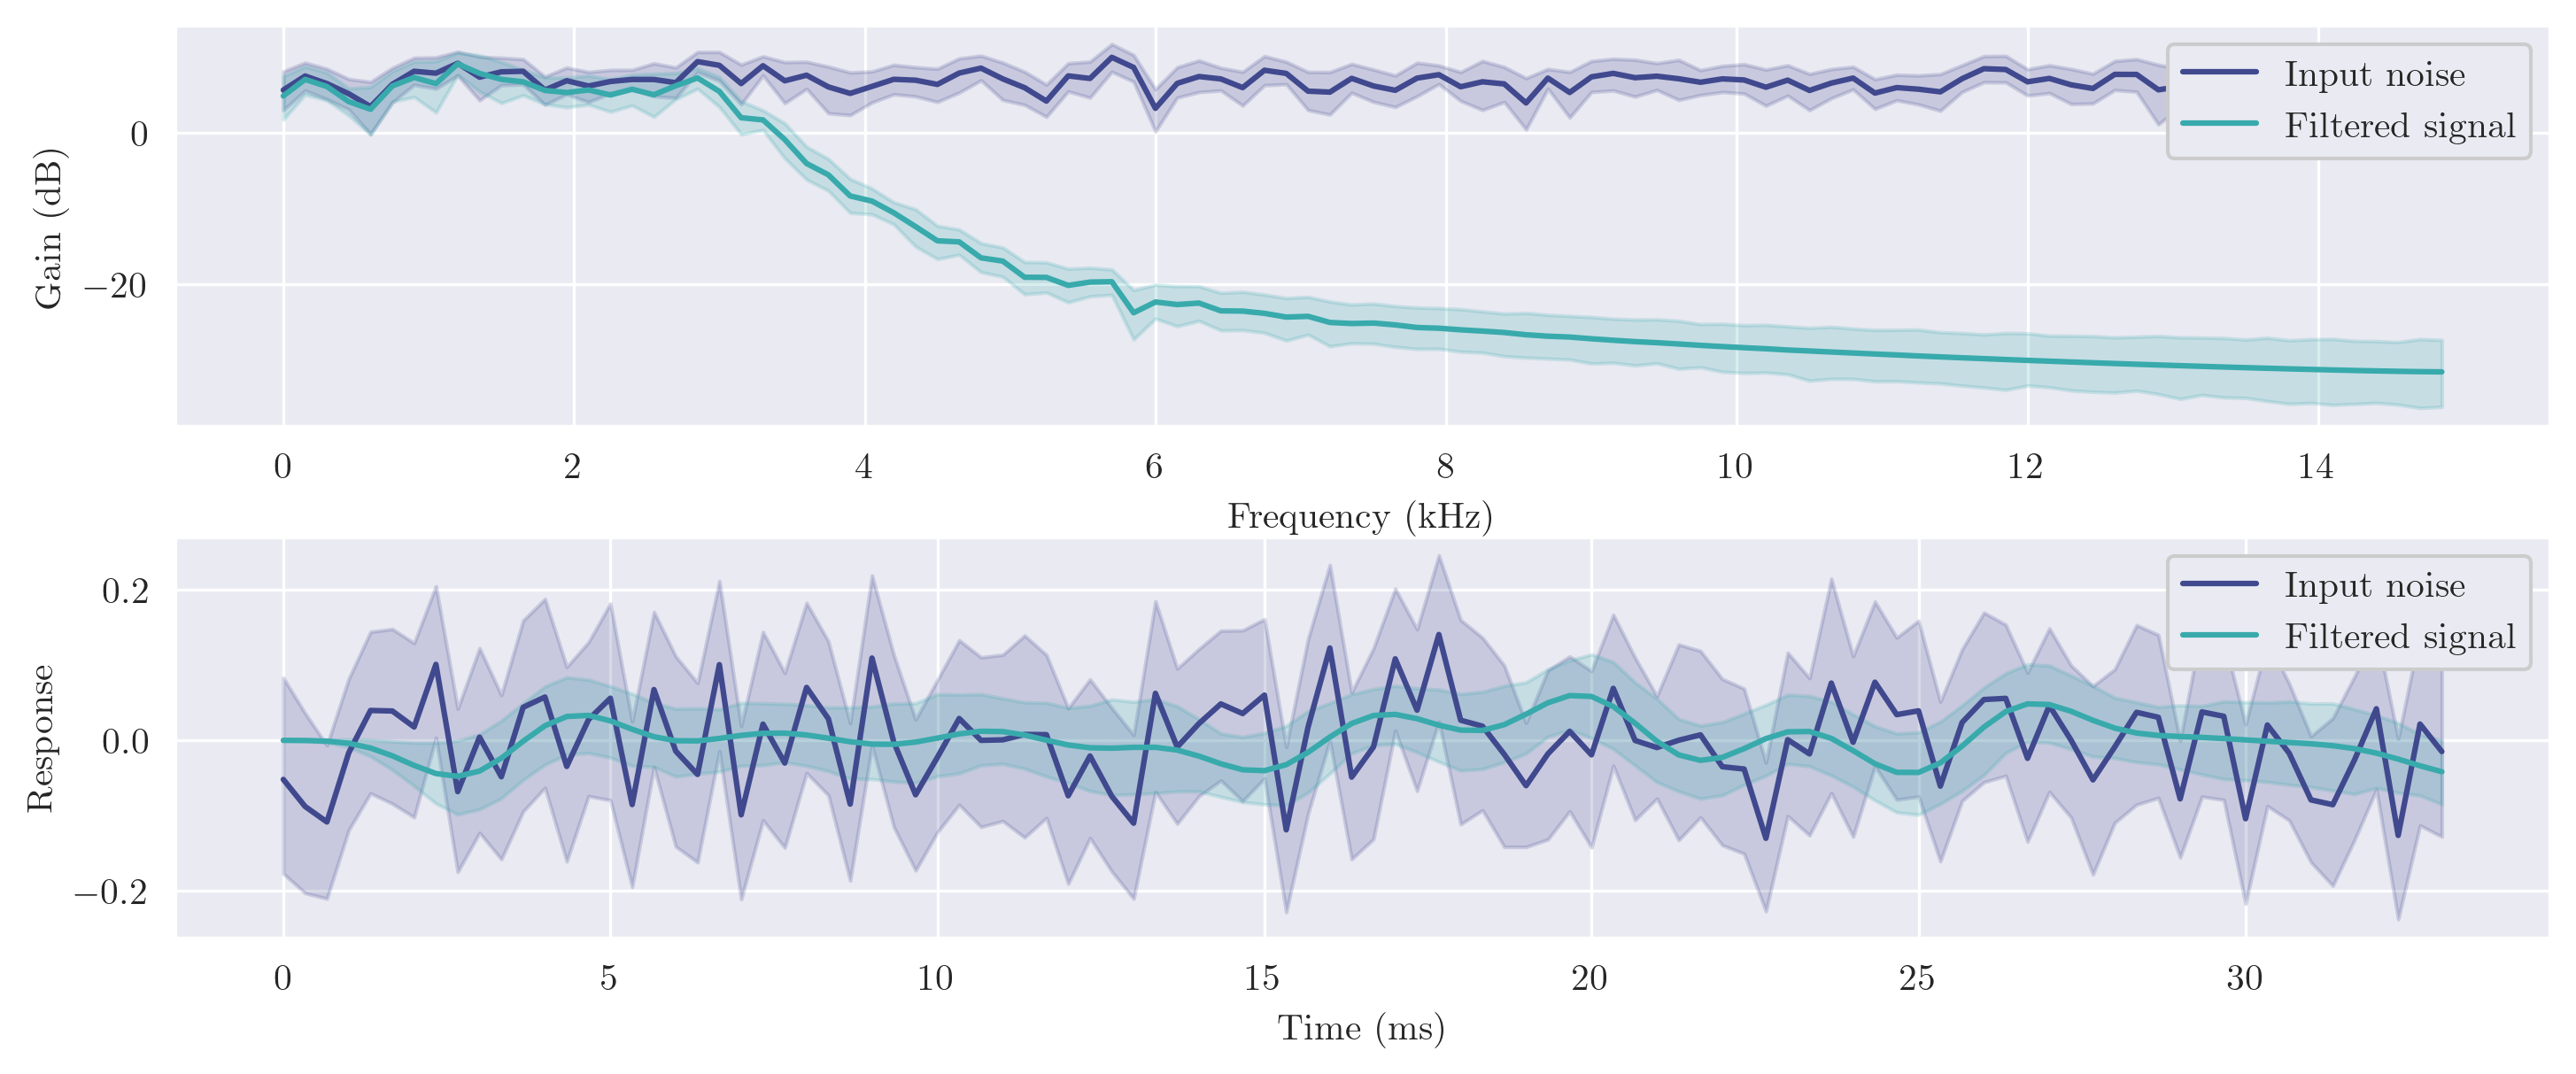
\includegraphics[width=0.99\textwidth]{images/q8_6th_stability.png}
    \caption{Original and (6th-order) filtered noise signals using unquantized coefficients}
\end{figure}

\begin{figure}[!ht]
    \centering
    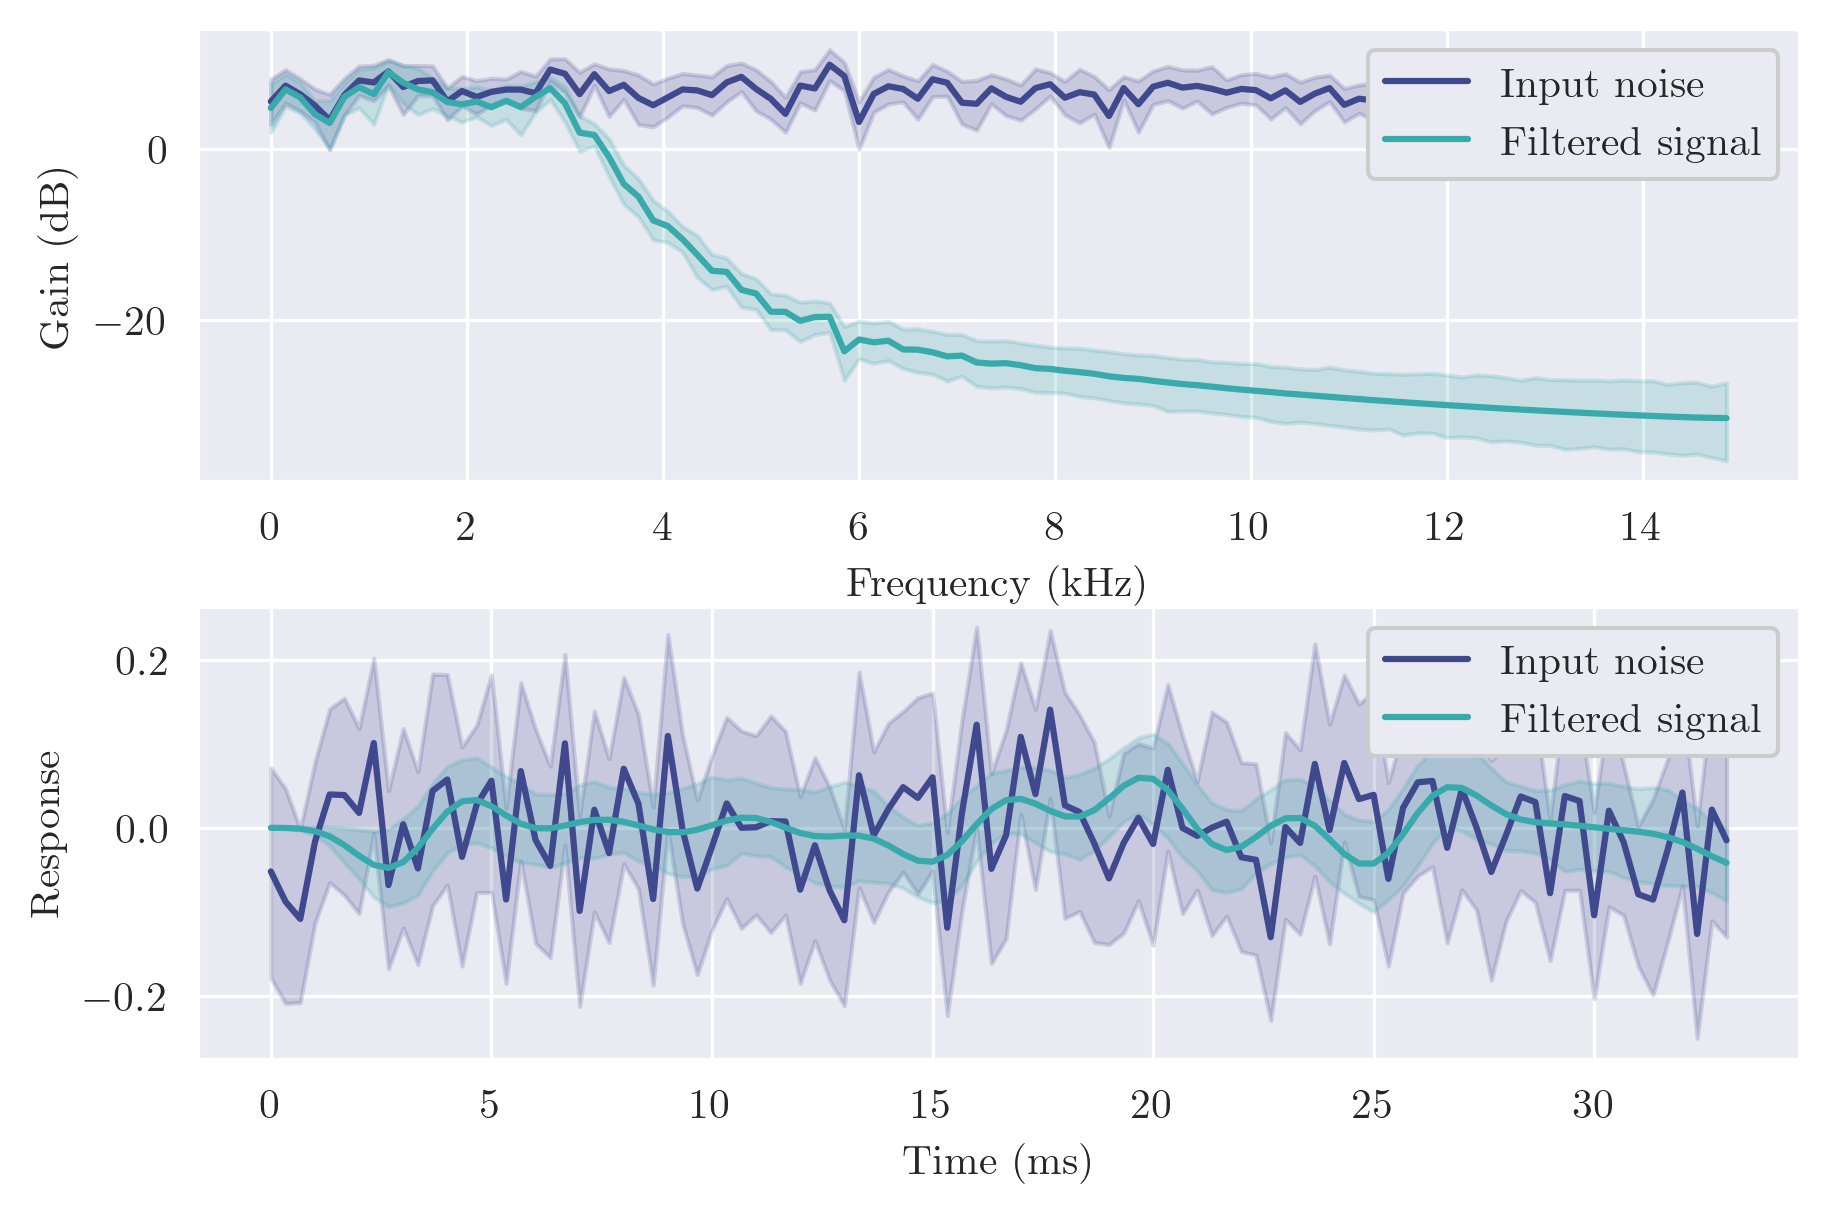
\includegraphics[width=0.99\textwidth]{images/q8_q6th_stability.png}
    \caption{Original and (6th-order) filtered noise signals using quantized coefficients}
\end{figure}

\newpage
{\Large\textbf{Filter Order: 7 (Unquantized and Quantized)}}
\vfill

\begin{figure}[ht]
    \centering
    \begin{subfigure}[b]{0.53\textwidth}
        \centering
        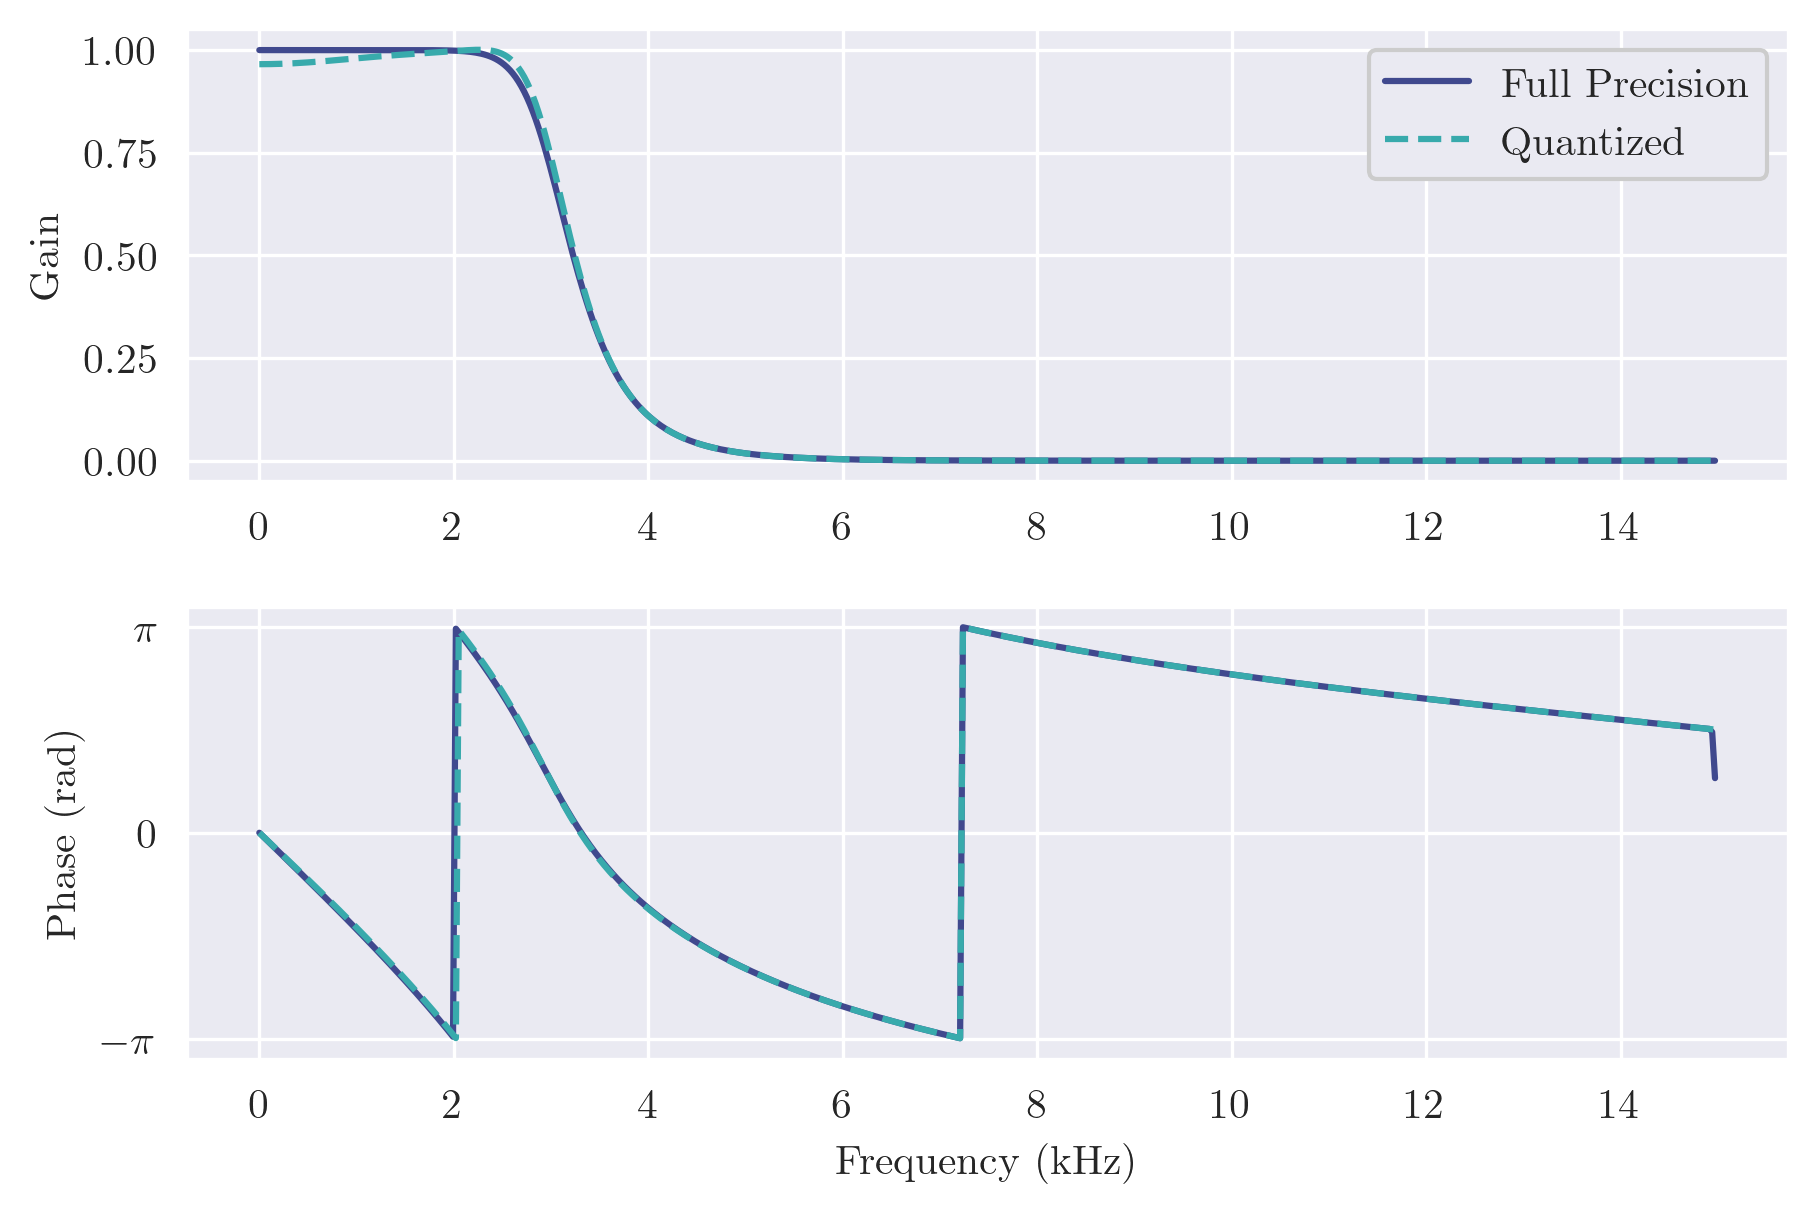
\includegraphics[width=\textwidth]{images/q8_7th_freqz.png}
    \end{subfigure}
    \hfill
    \begin{subfigure}[b]{0.46\textwidth}
        \centering
        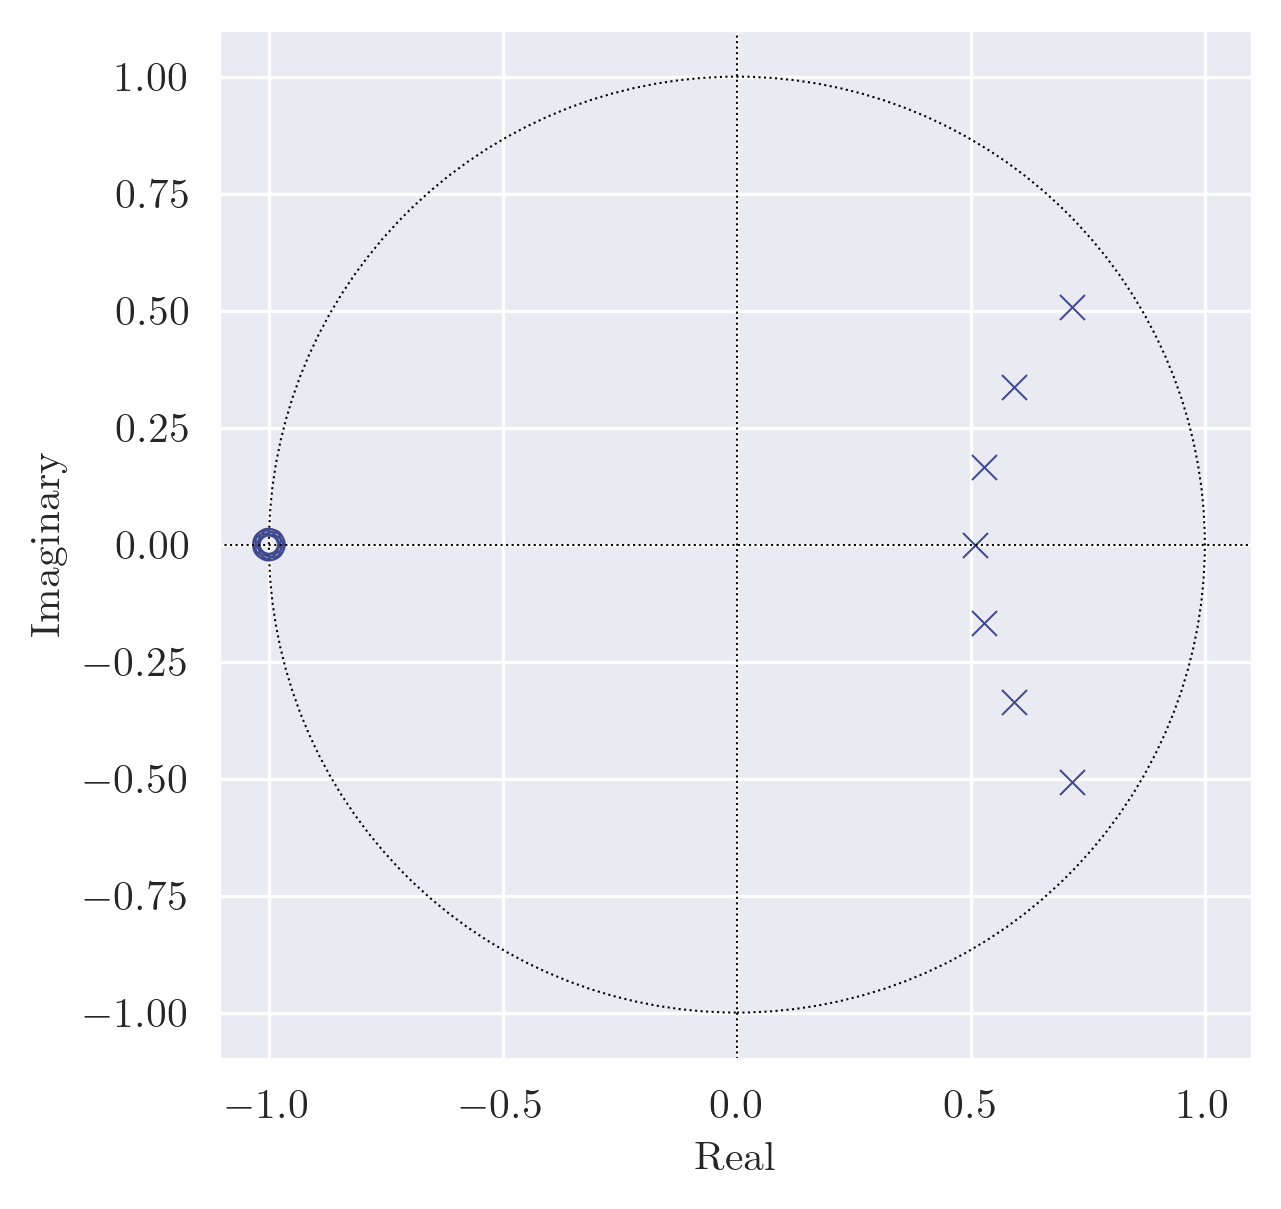
\includegraphics[width=\textwidth]{images/q8_7th_zp.png}
    \end{subfigure}
    \caption{Frequency response and pole-zero plot of 7th-order low pass Butterworth filter}
\end{figure}

\begin{figure}[!ht]
    \centering
    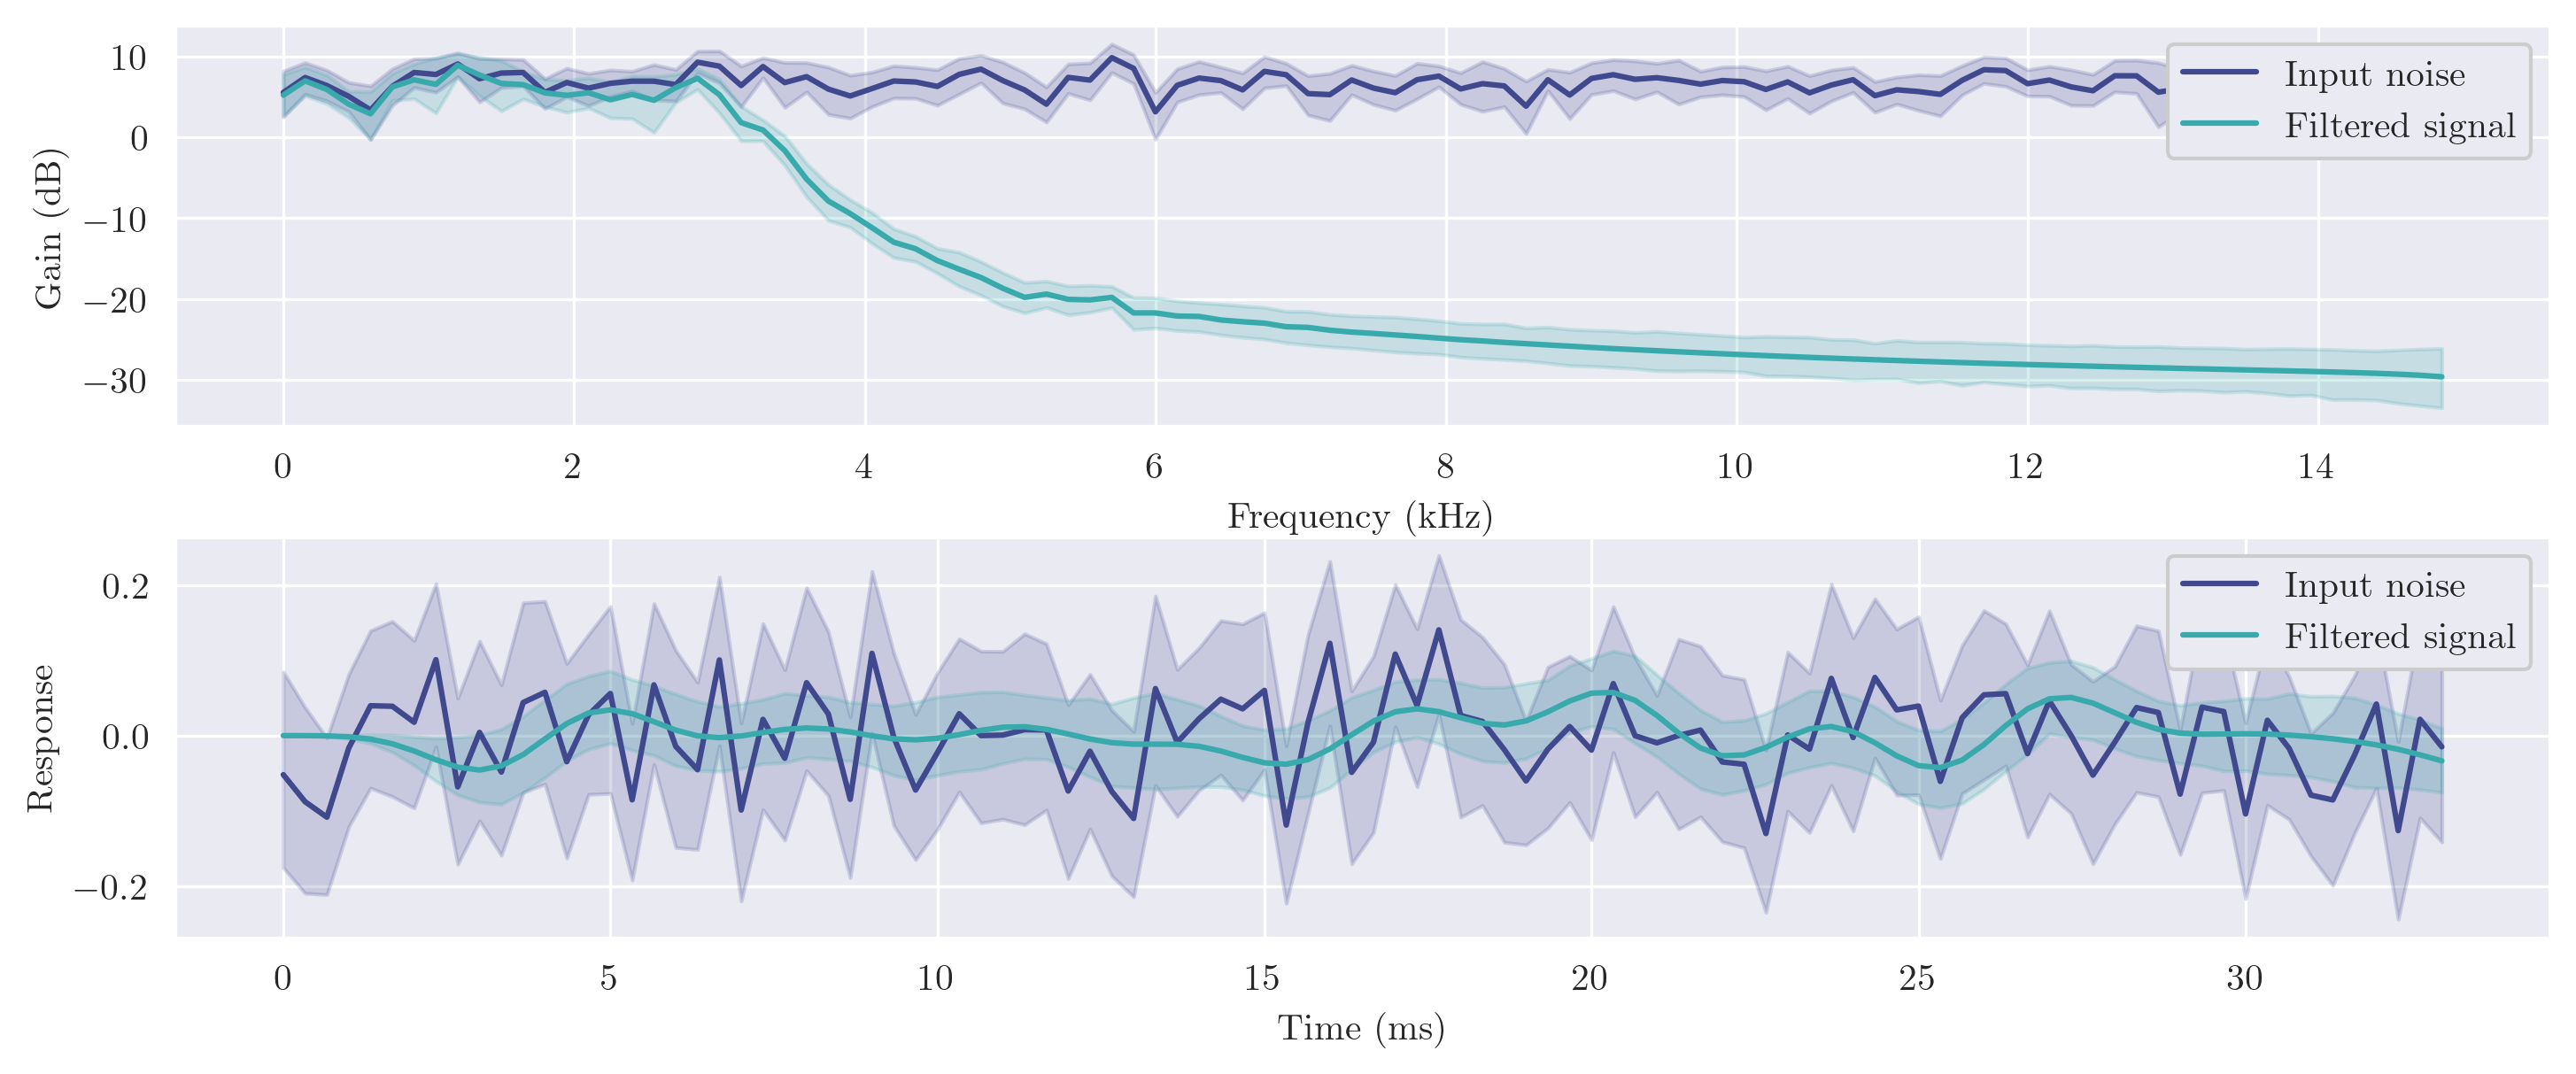
\includegraphics[width=0.99\textwidth]{images/q8_7th_stability.png}
    \caption{Original and (7th-order) filtered noise signals using unquantized coefficients}
\end{figure}

\begin{figure}[!ht]
    \centering
    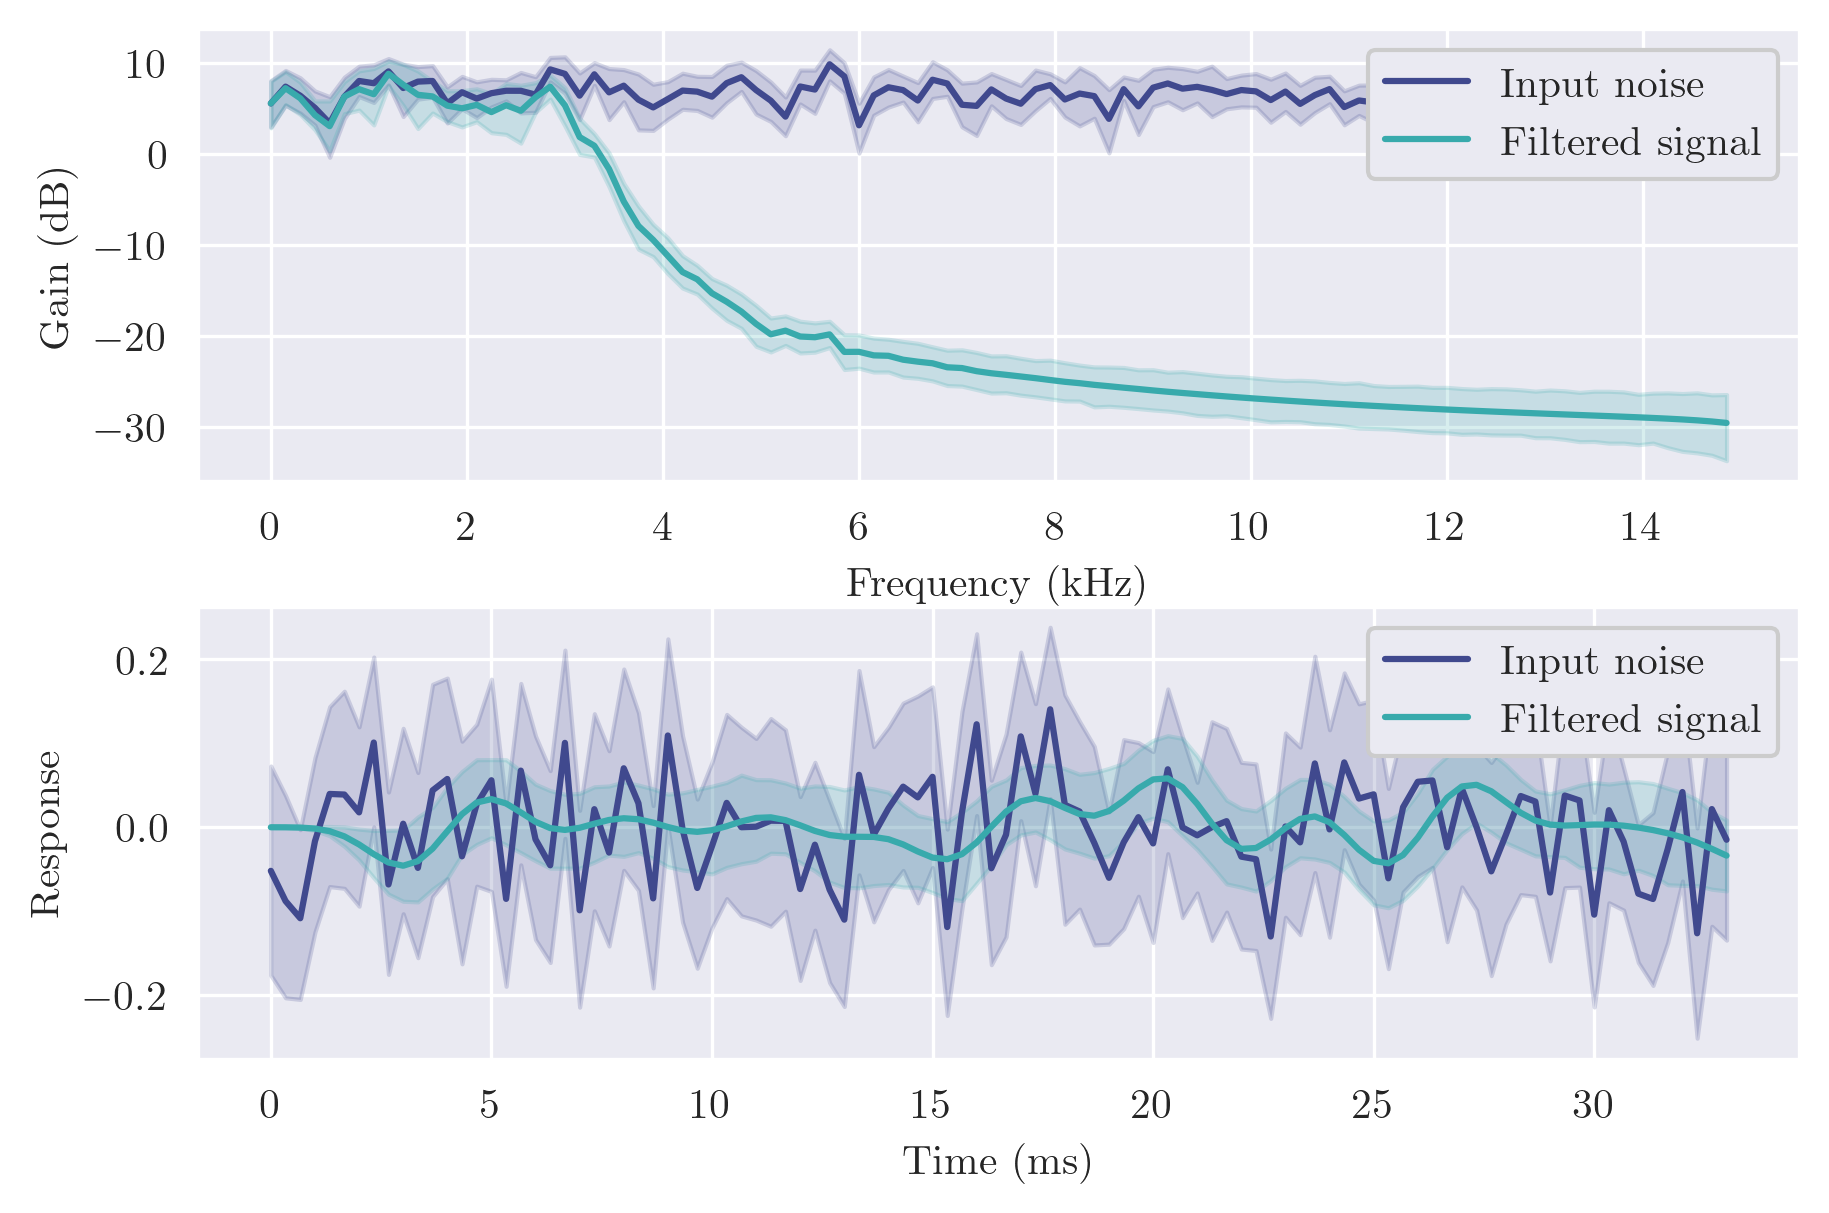
\includegraphics[width=0.99\textwidth]{images/q8_q7th_stability.png}
    \caption{Original and (7th-order) filtered noise signals using quantized coefficients}
\end{figure}

\newpage
{\Large\textbf{Filter Order: 8 (Unquantized and Quantized)}}
\vfill

\begin{figure}[ht]
    \centering
    \begin{subfigure}[b]{0.52\textwidth}
        \centering
        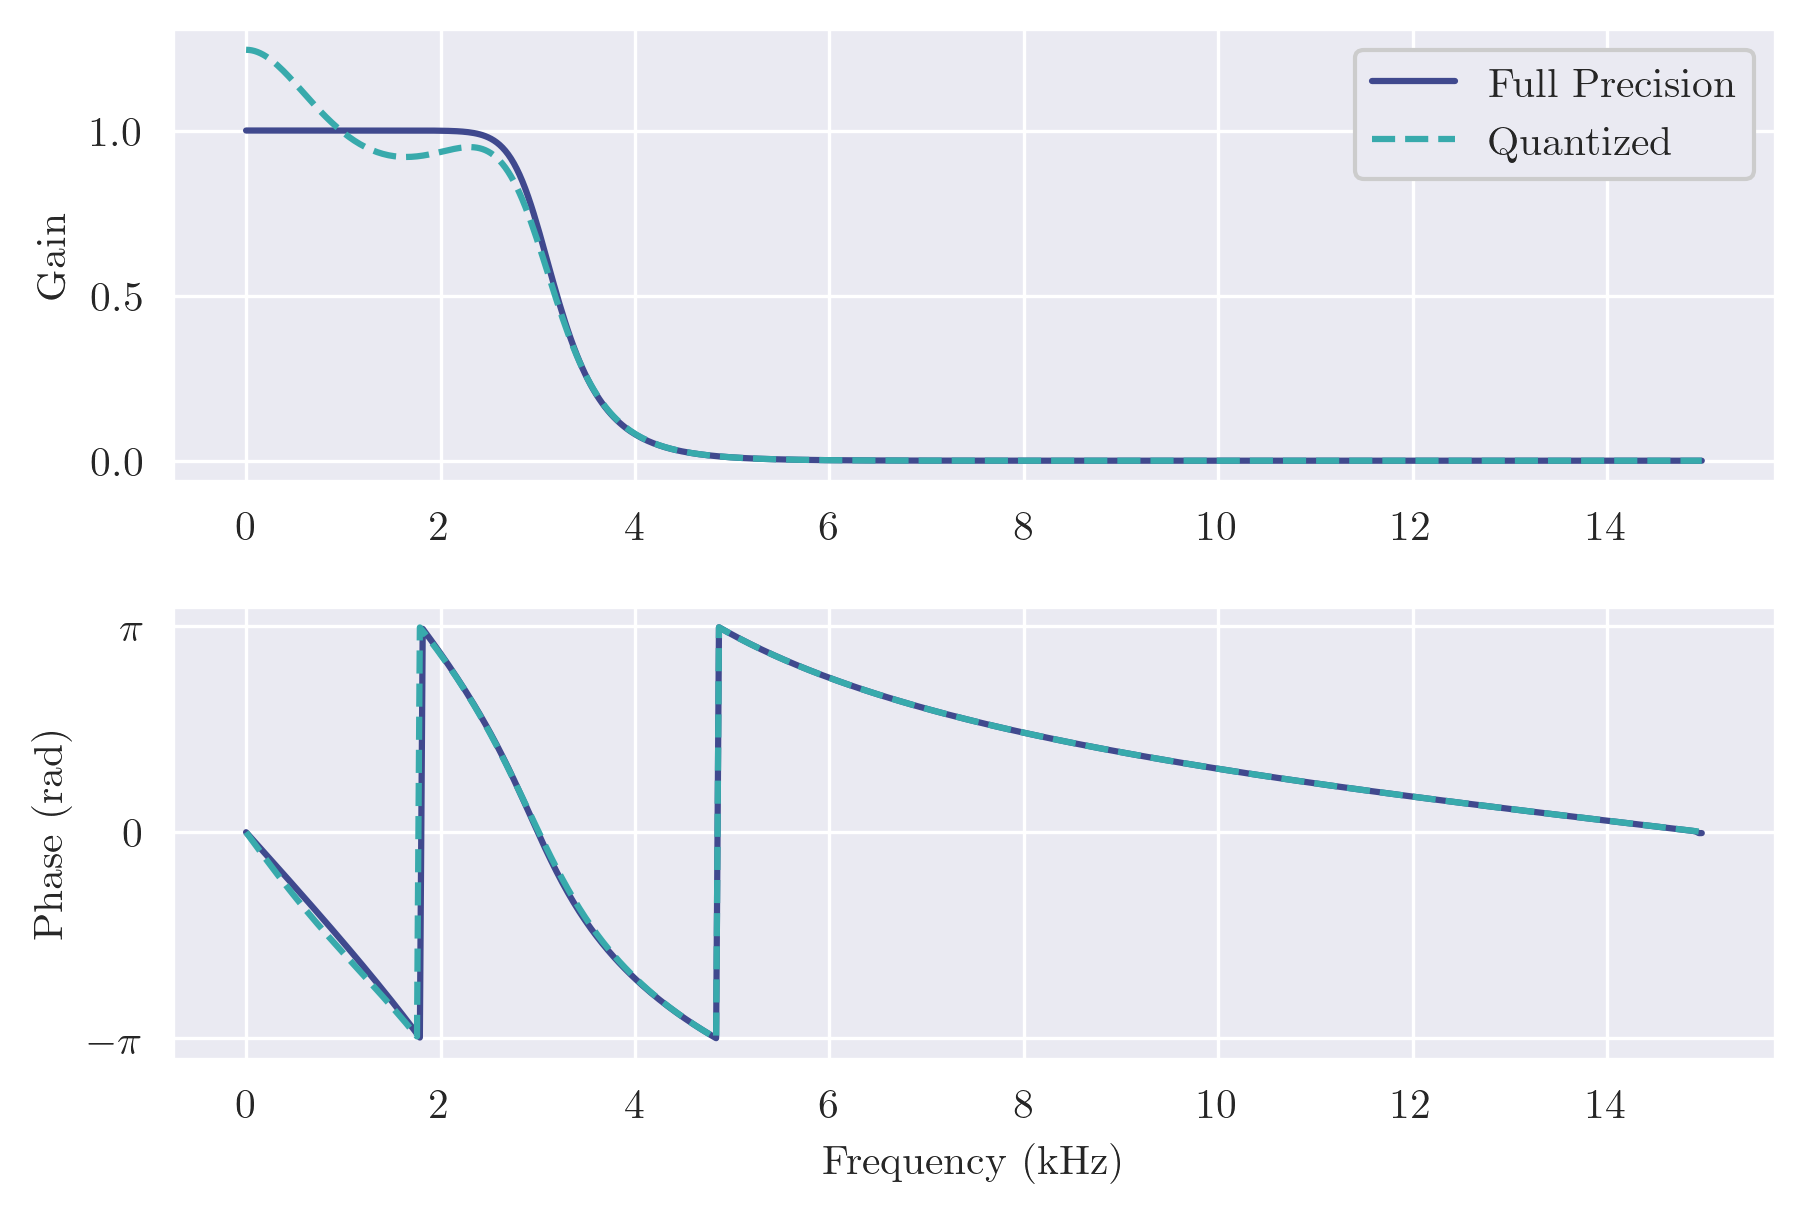
\includegraphics[width=\textwidth]{images/q8_8th_freqz.png}
    \end{subfigure}
    \hfill
    \begin{subfigure}[b]{0.47\textwidth}
        \centering
        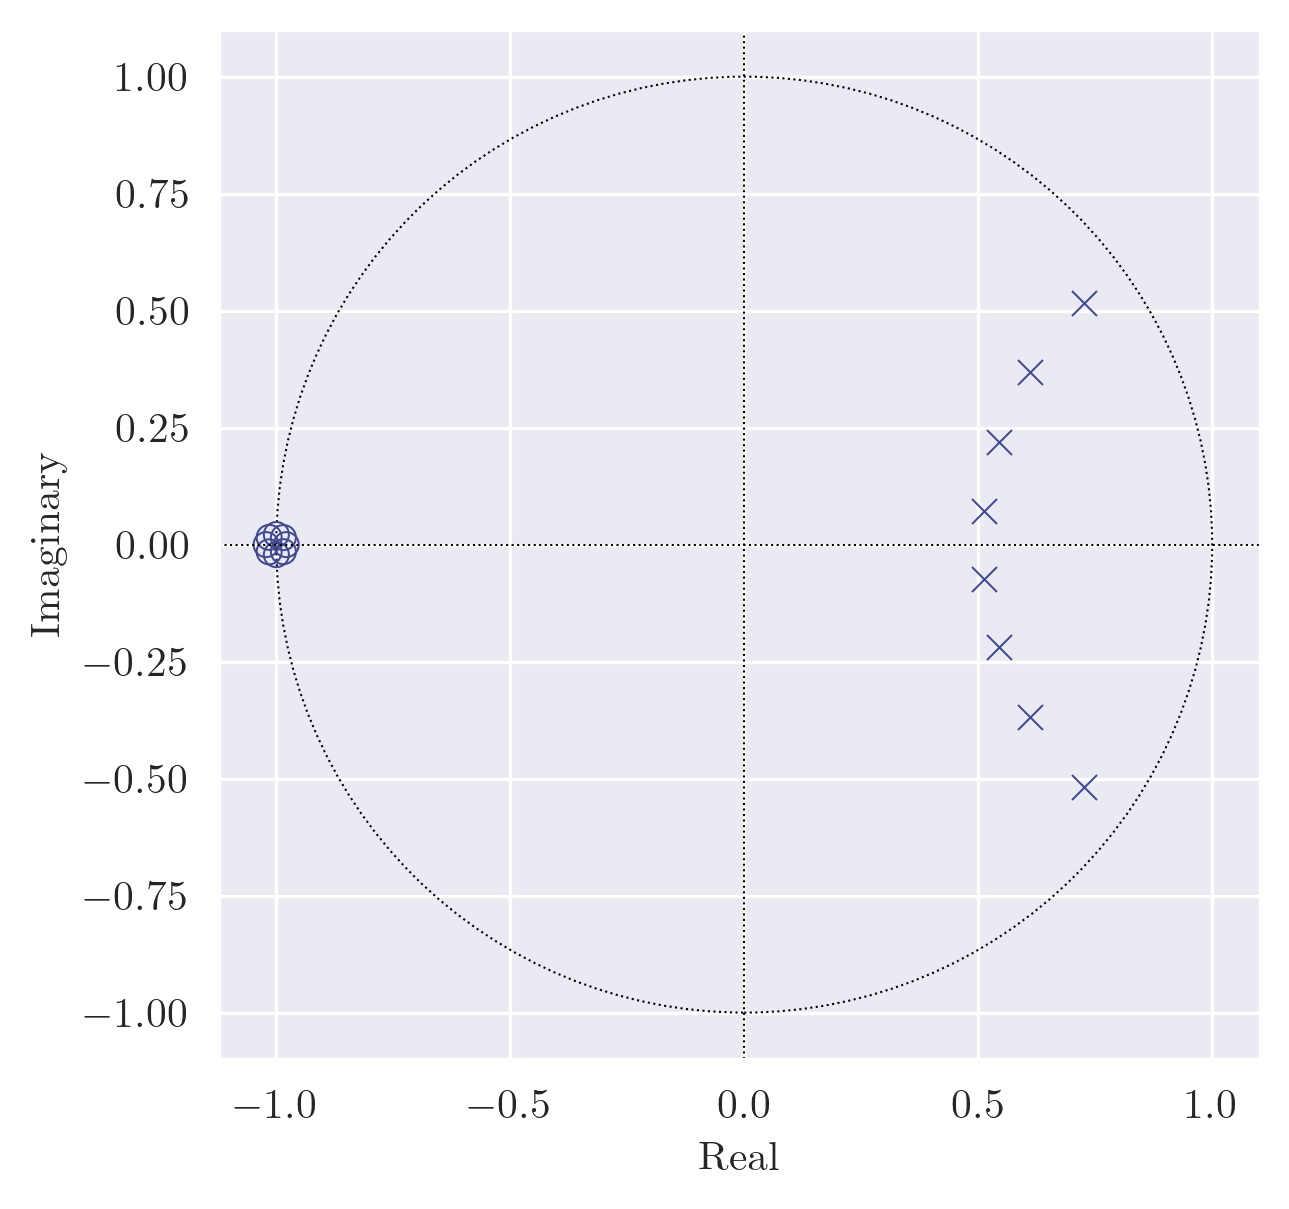
\includegraphics[width=\textwidth]{images/q8_8th_zp.png}
    \end{subfigure}
    \caption{Frequency response and pole-zero plot of 8th-order low pass Butterworth filter}
\end{figure}

\begin{figure}[!ht]
    \centering
    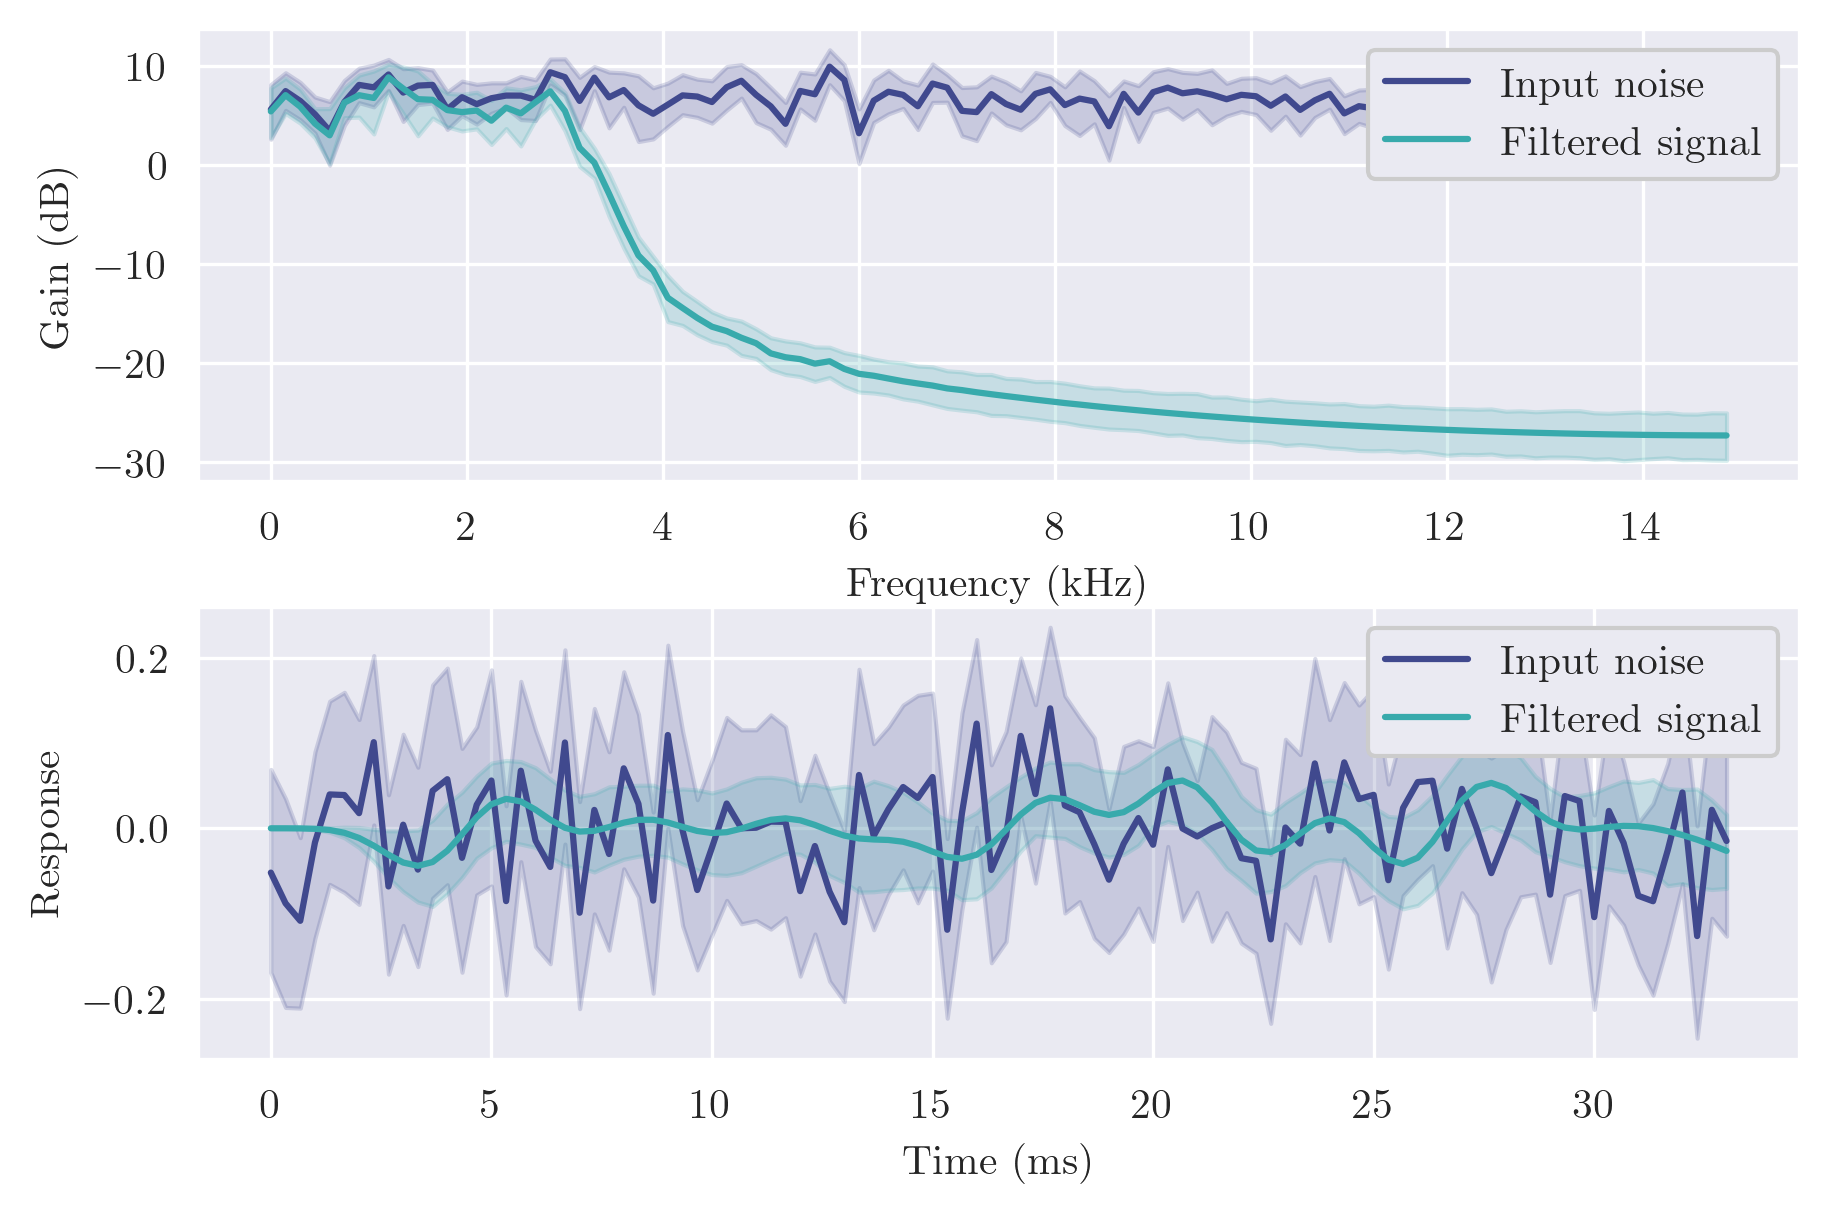
\includegraphics[width=0.99\textwidth]{images/q8_8th_stability.png}
    \caption{Original and (8th-order) filtered noise signals using unquantized coefficients}
\end{figure}

\begin{figure}[!ht]
    \centering
    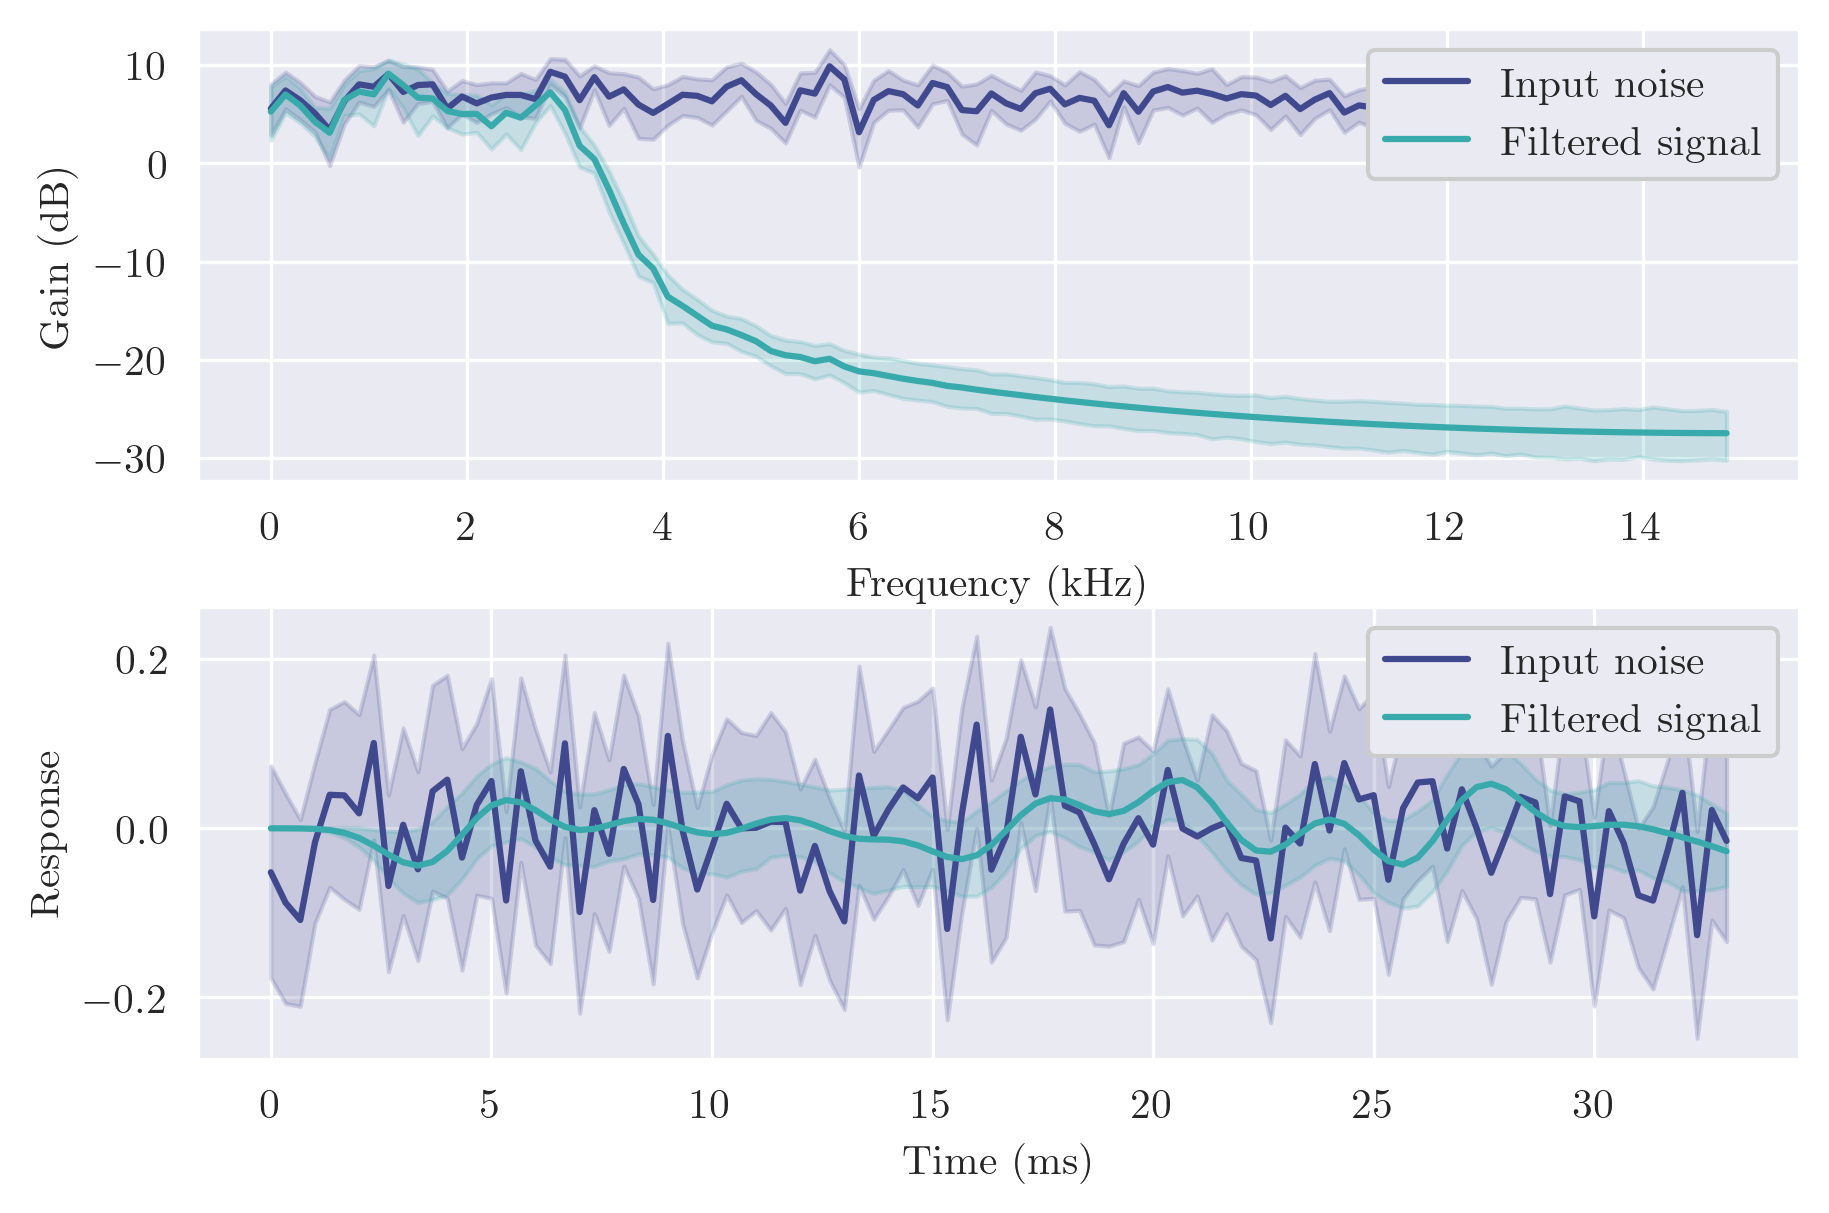
\includegraphics[width=0.99\textwidth]{images/q8_q8th_stability.png}
    \caption{Original and (8th-order) filtered noise signals using quantized coefficients}
\end{figure}

\newpage
{\Large\textbf{Filter Order: 10 (Quantized)}}
\vspace{1em}

\begin{figure}[ht]
    \centering
    \begin{subfigure}[b]{0.51\textwidth}
        \centering
        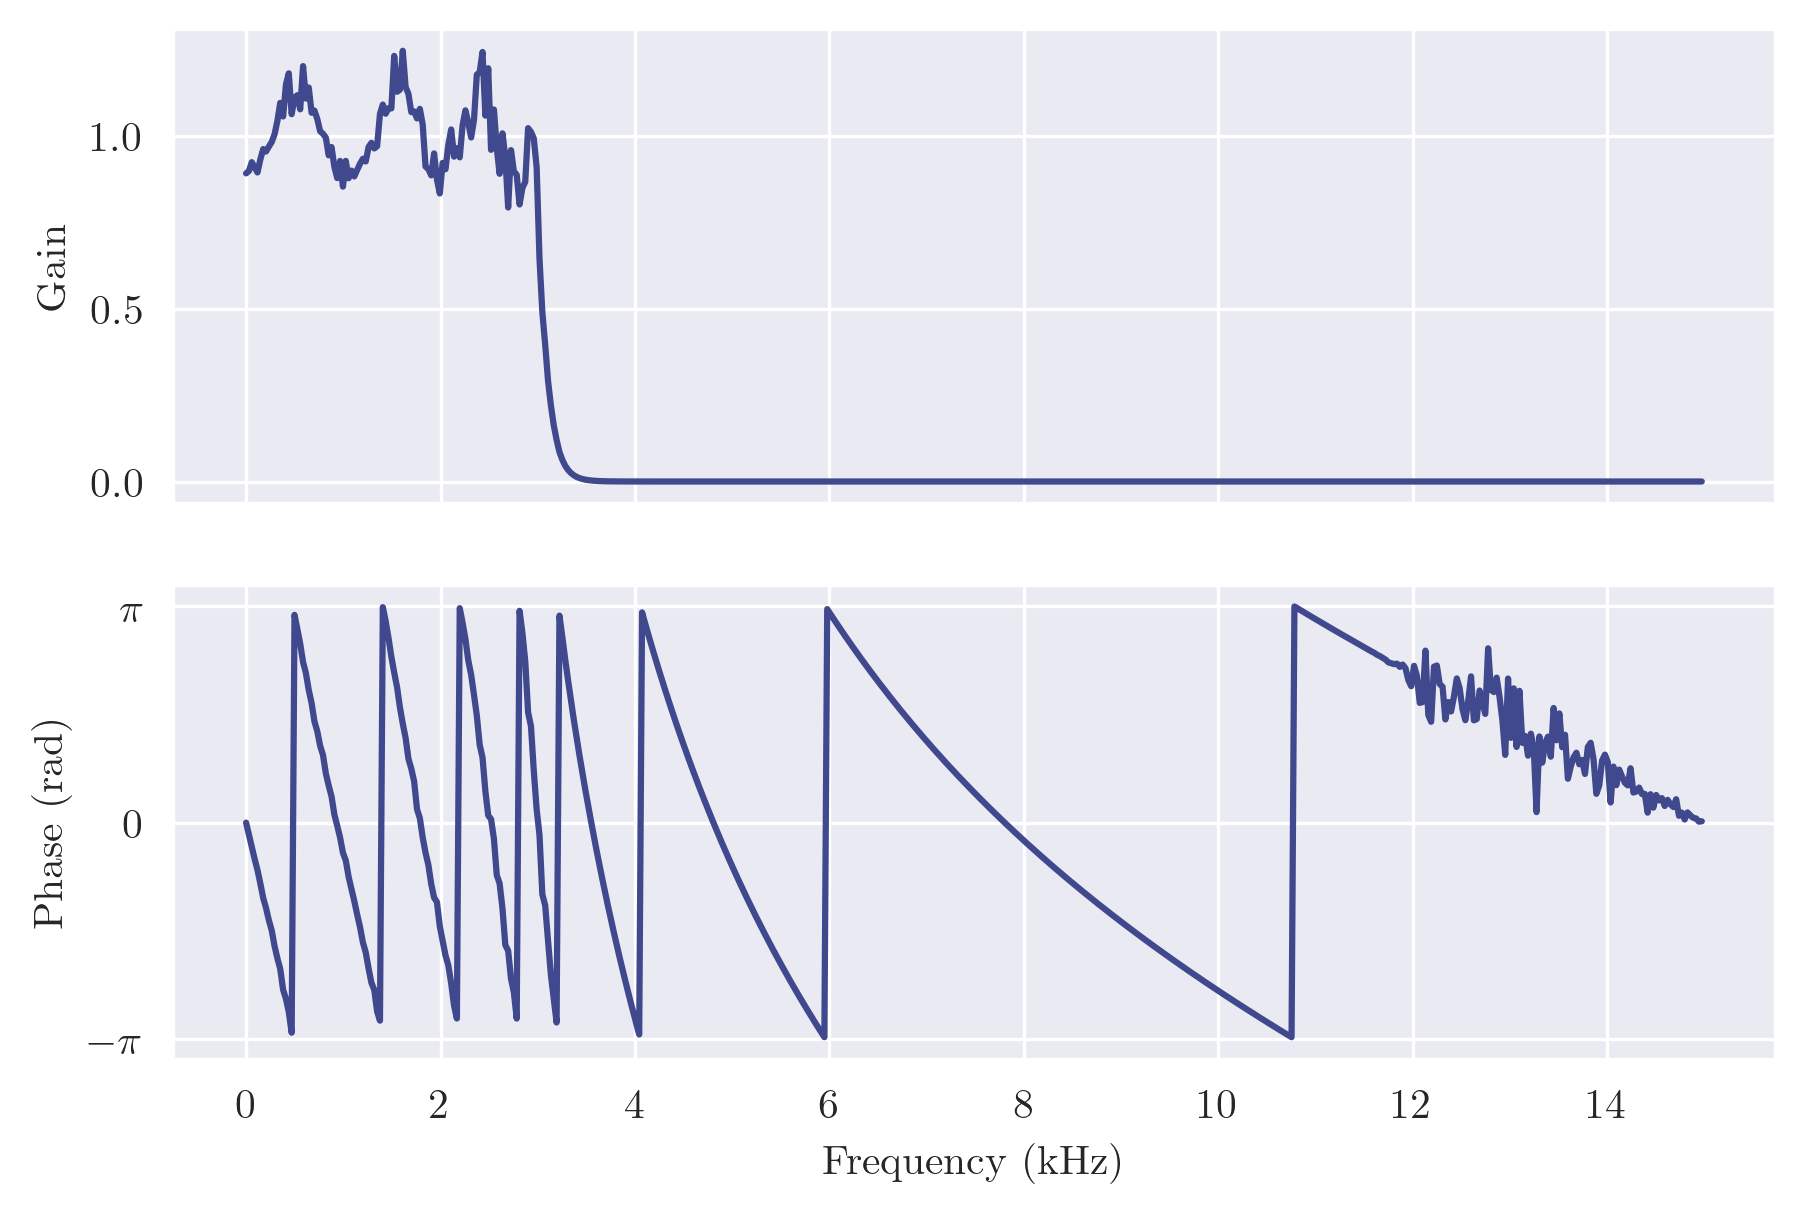
\includegraphics[width=\textwidth]{images/q8_q10th_freqz.png}
    \end{subfigure}
    \hfill
    \begin{subfigure}[b]{0.48\textwidth}
        \centering
        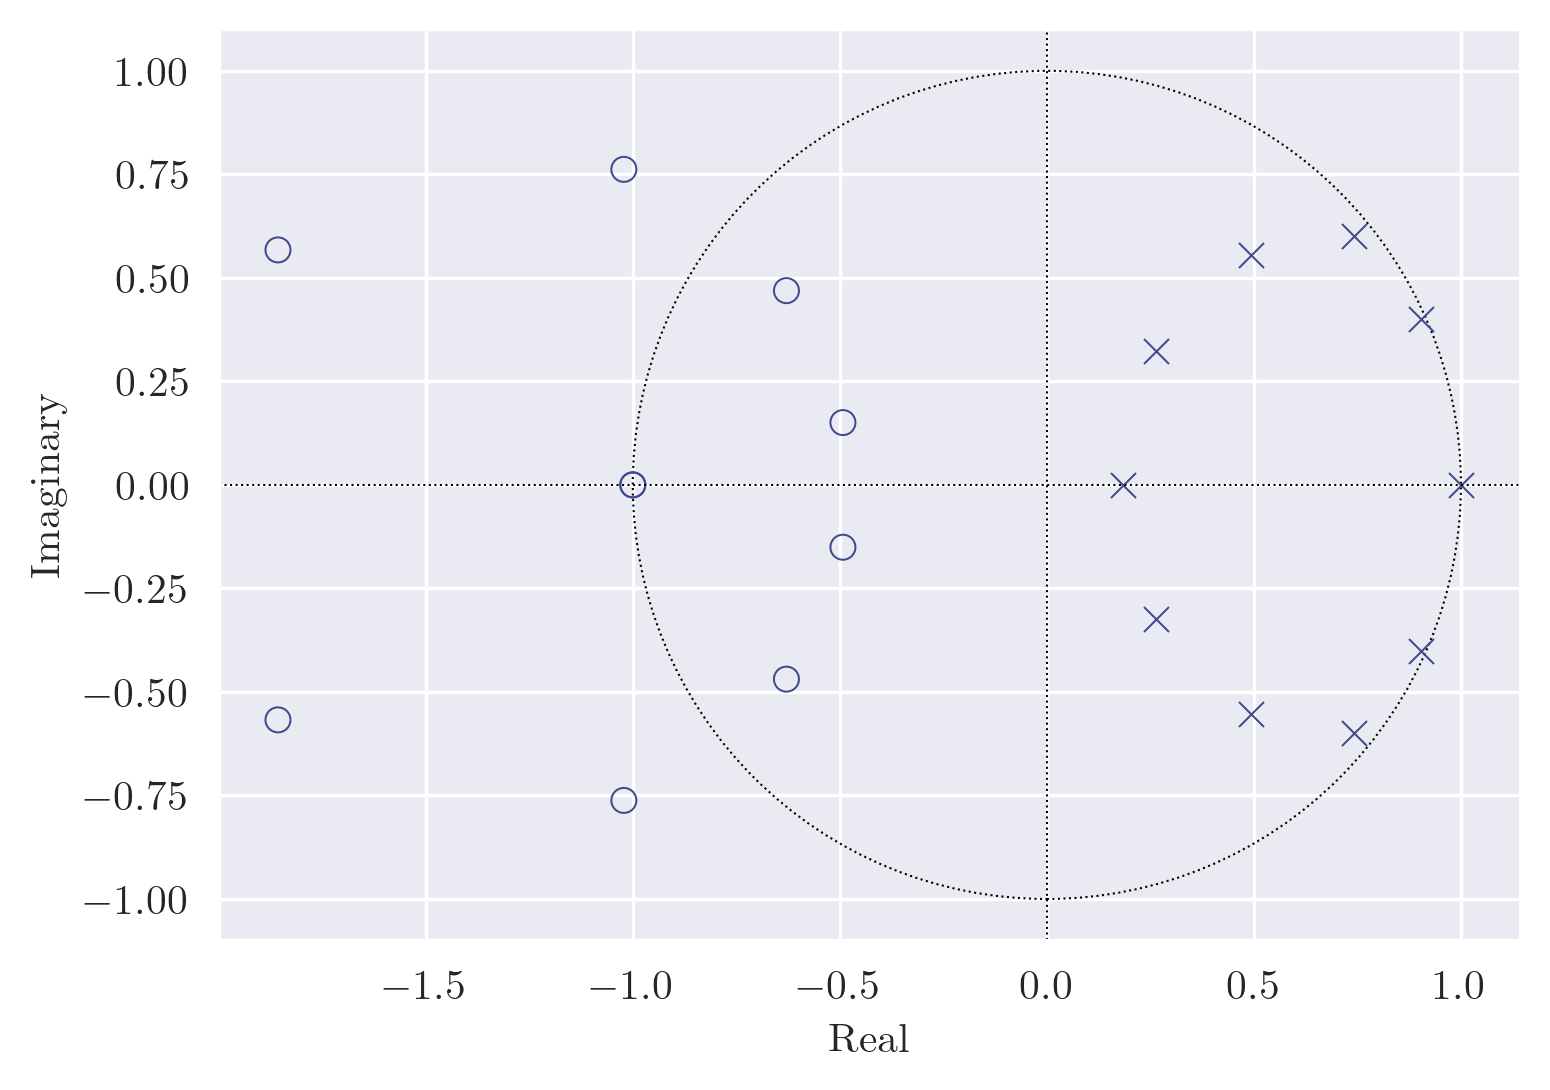
\includegraphics[width=\textwidth]{images/q8_q10th_zp.png}
    \end{subfigure}
    \caption{Frequency response and pole-zero plot of 10th-order low pass Butterworth filter}
\end{figure}

\begin{figure}[!ht]
    \centering
    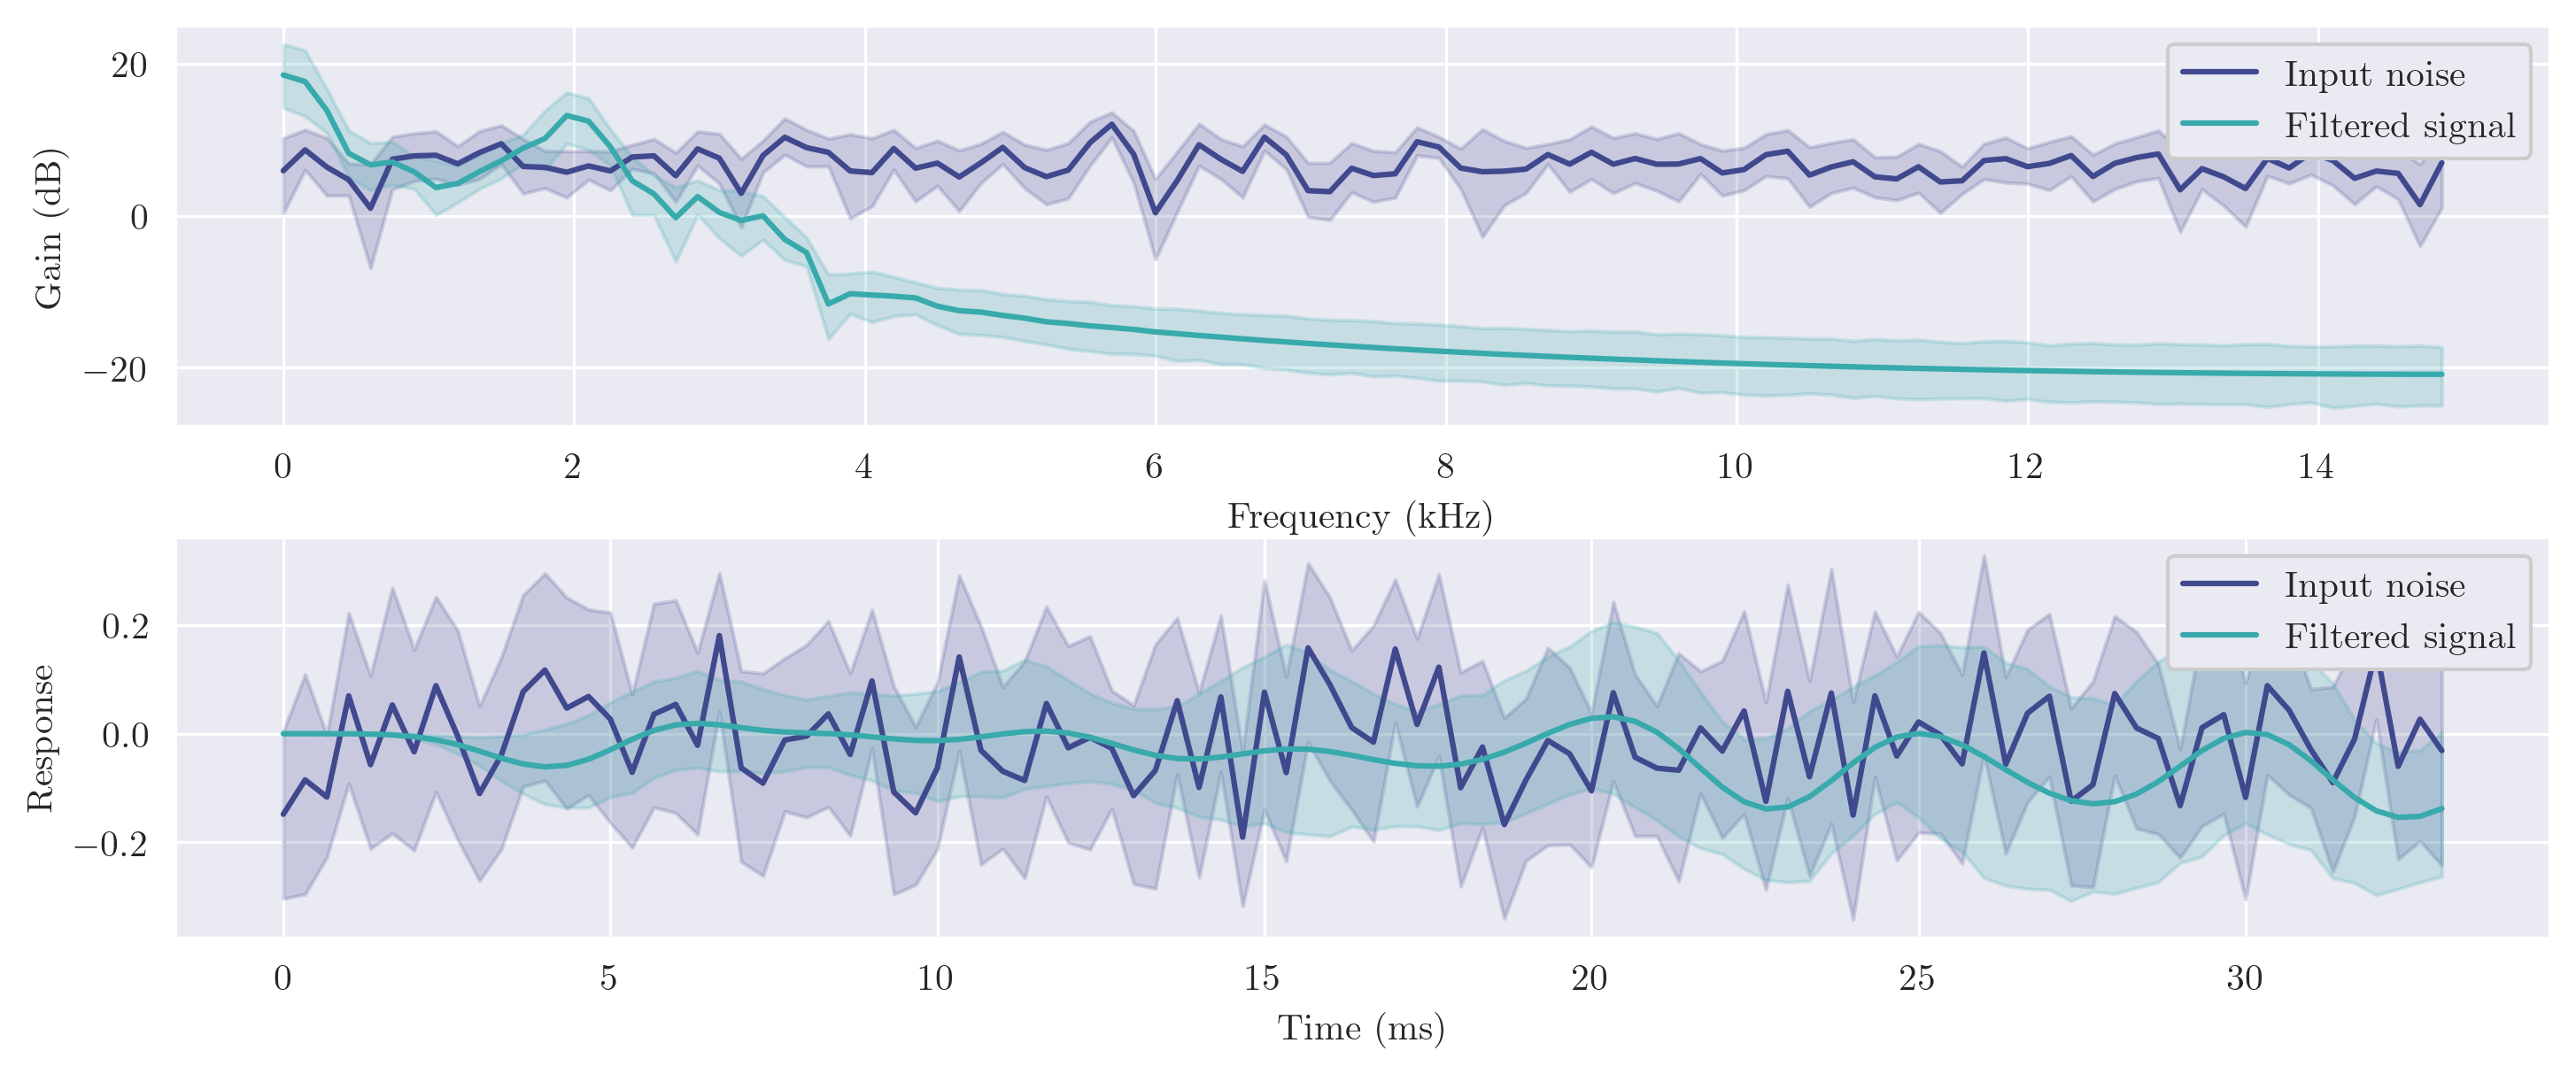
\includegraphics[width=0.99\textwidth]{images/q8_q10th_stability.png}
    \caption{Original and (10th-order) filtered noise signals using quantized coefficients}
\end{figure}

\newpage
{\Large\textbf{Filter Order: 11 (Quantized)}}
\vspace{1em}

\begin{figure}[ht]
    \centering
    \begin{subfigure}[b]{0.47\textwidth}
        \centering
        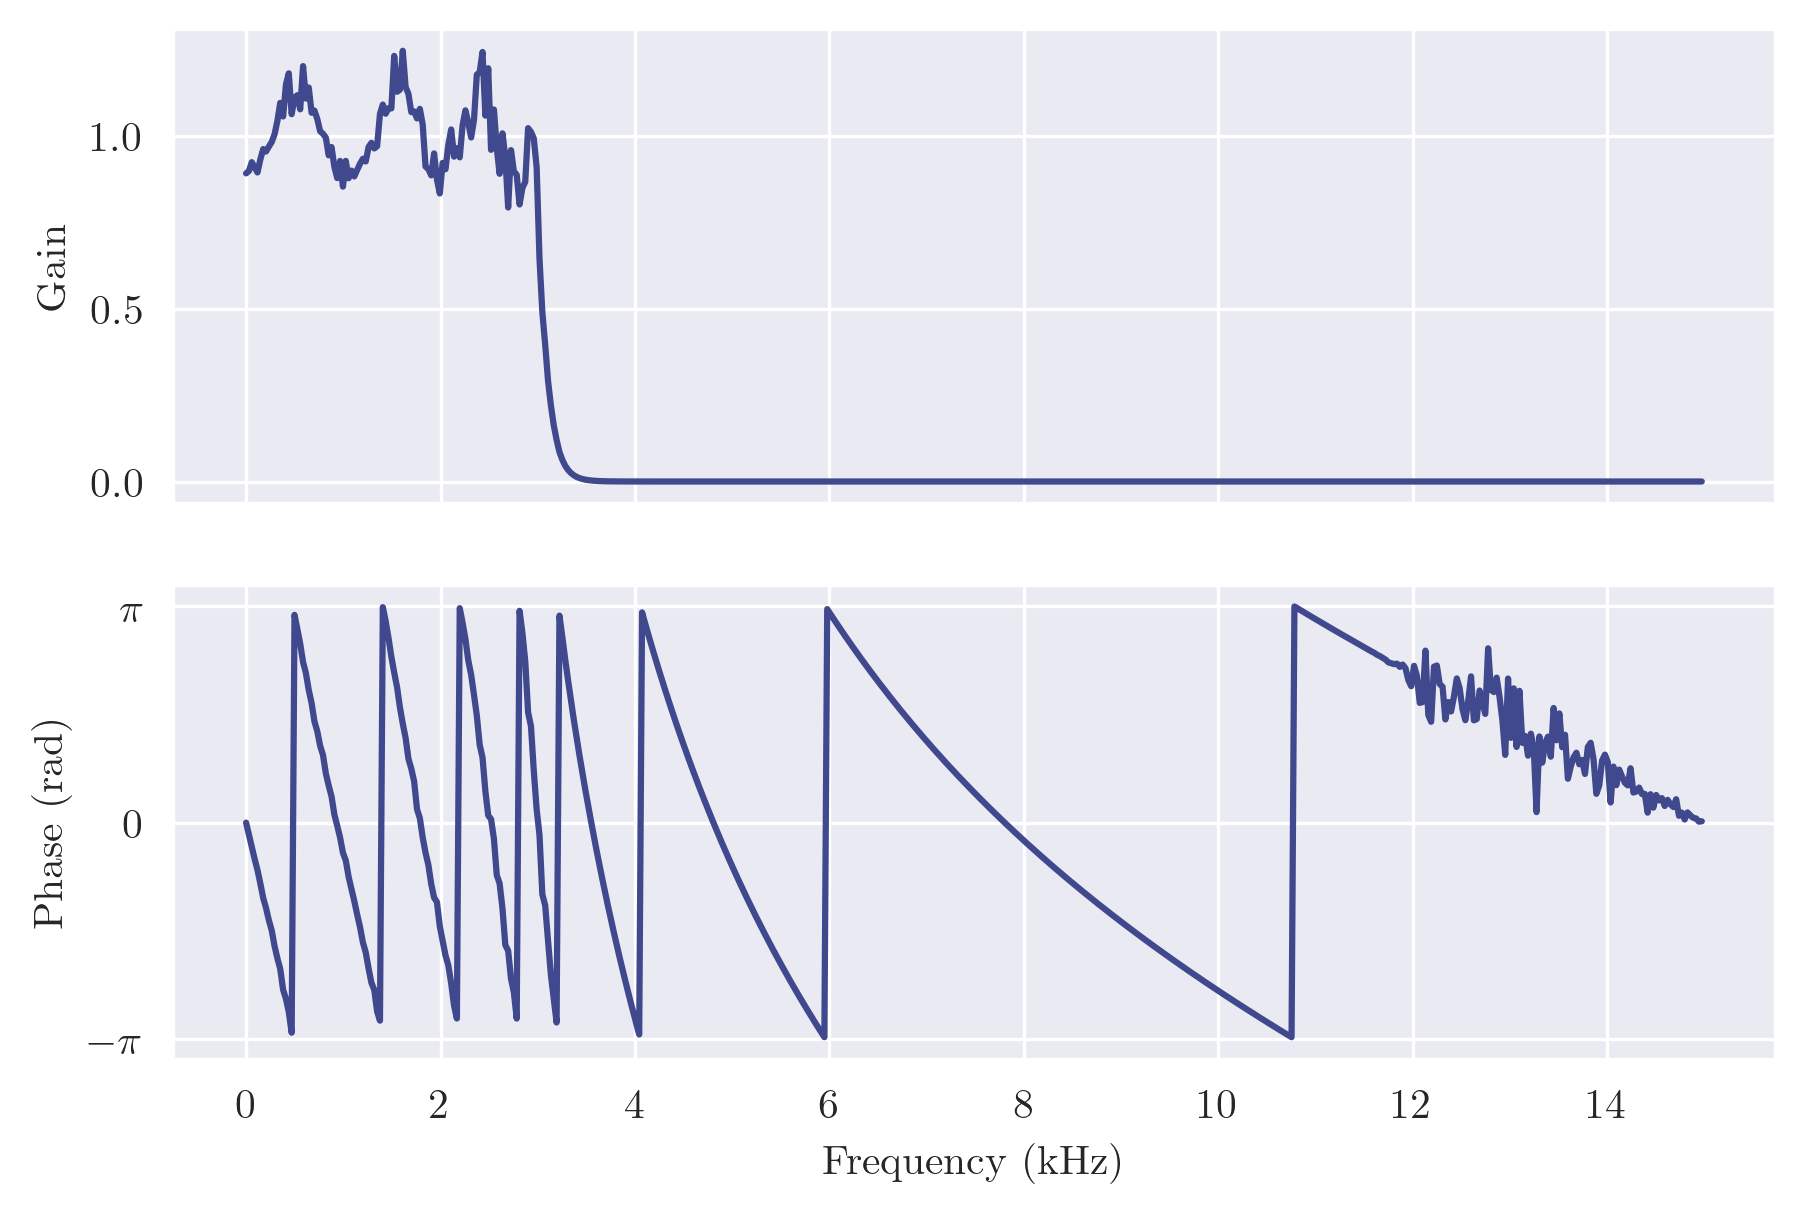
\includegraphics[width=\textwidth]{images/q8_q11th_freqz.png}
    \end{subfigure}
    \hfill
    \begin{subfigure}[b]{0.52\textwidth}
        \centering
        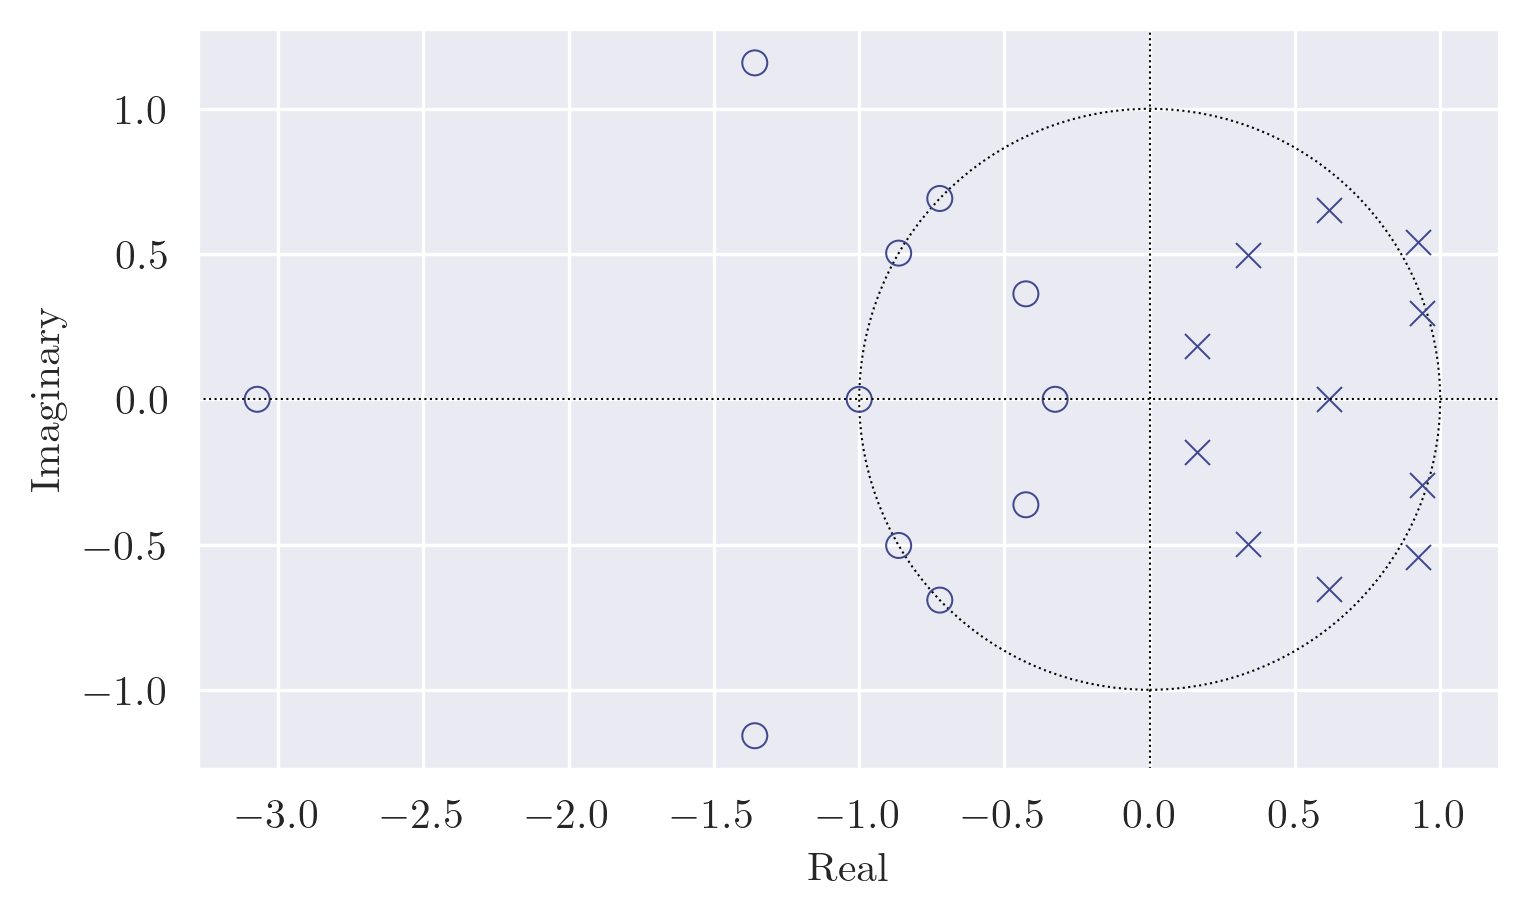
\includegraphics[width=\textwidth]{images/q8_q11th_zp.png}
    \end{subfigure}
    \caption{Frequency response and pole-zero plot of 11th-order low pass Butterworth filter}
\end{figure}

\begin{figure}[!ht]
    \centering
    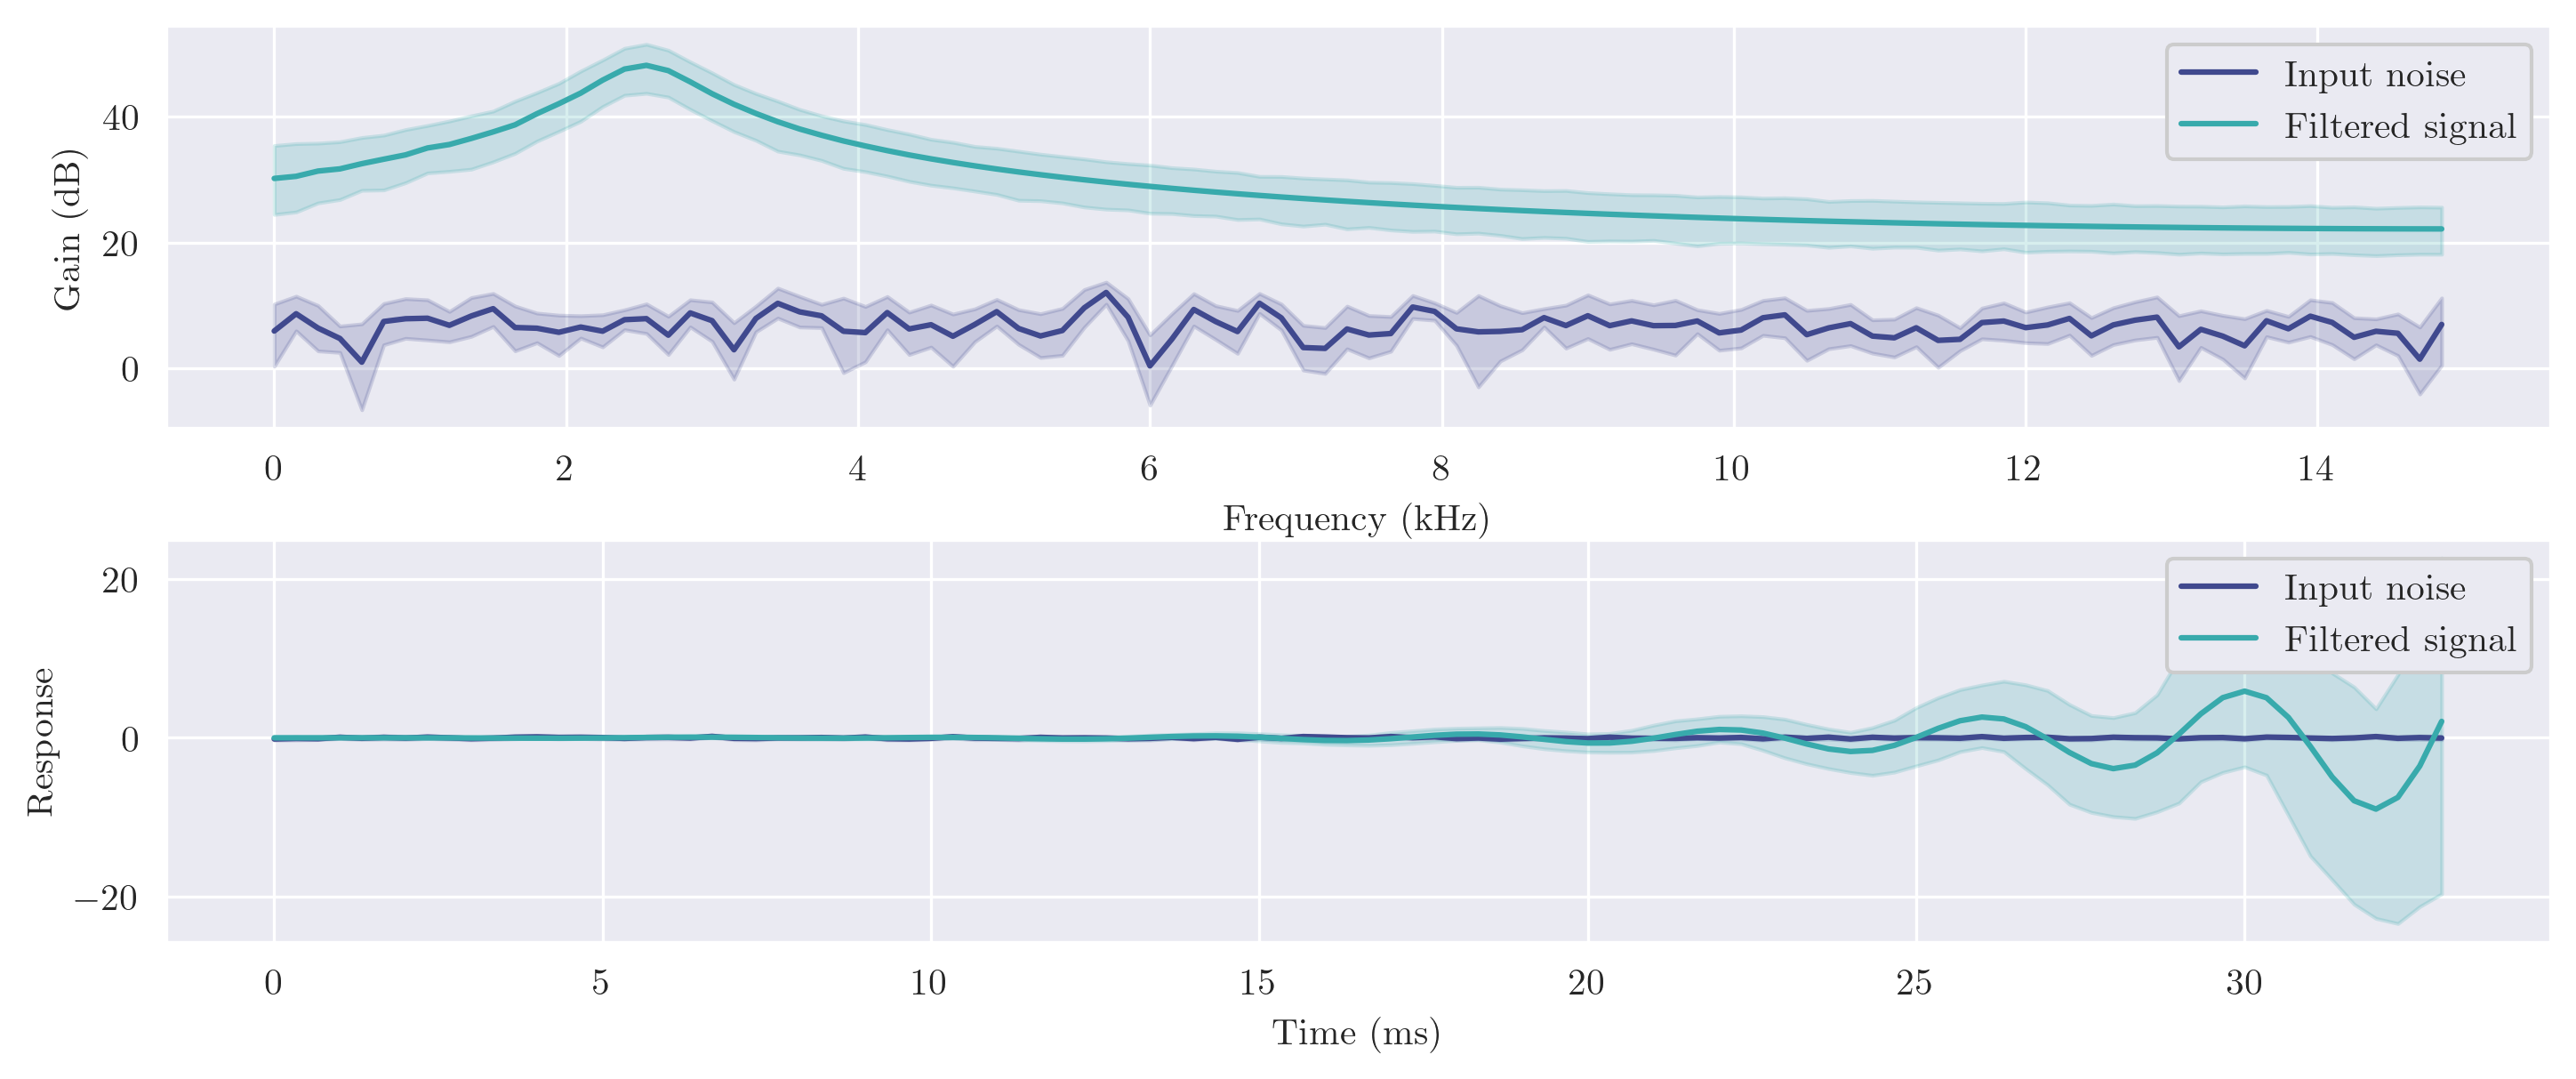
\includegraphics[width=0.99\textwidth]{images/q8_q11th_stability.png}
    \caption{Original and (11th-order) filtered noise signals using quantized coefficients}
\end{figure}

\newpage
{\Large\textbf{Filter Order: 31 (Unquantized)}}
\vspace{1em}

\begin{figure}[ht]
    \centering
    \begin{subfigure}[b]{0.71\textwidth}
        \centering
        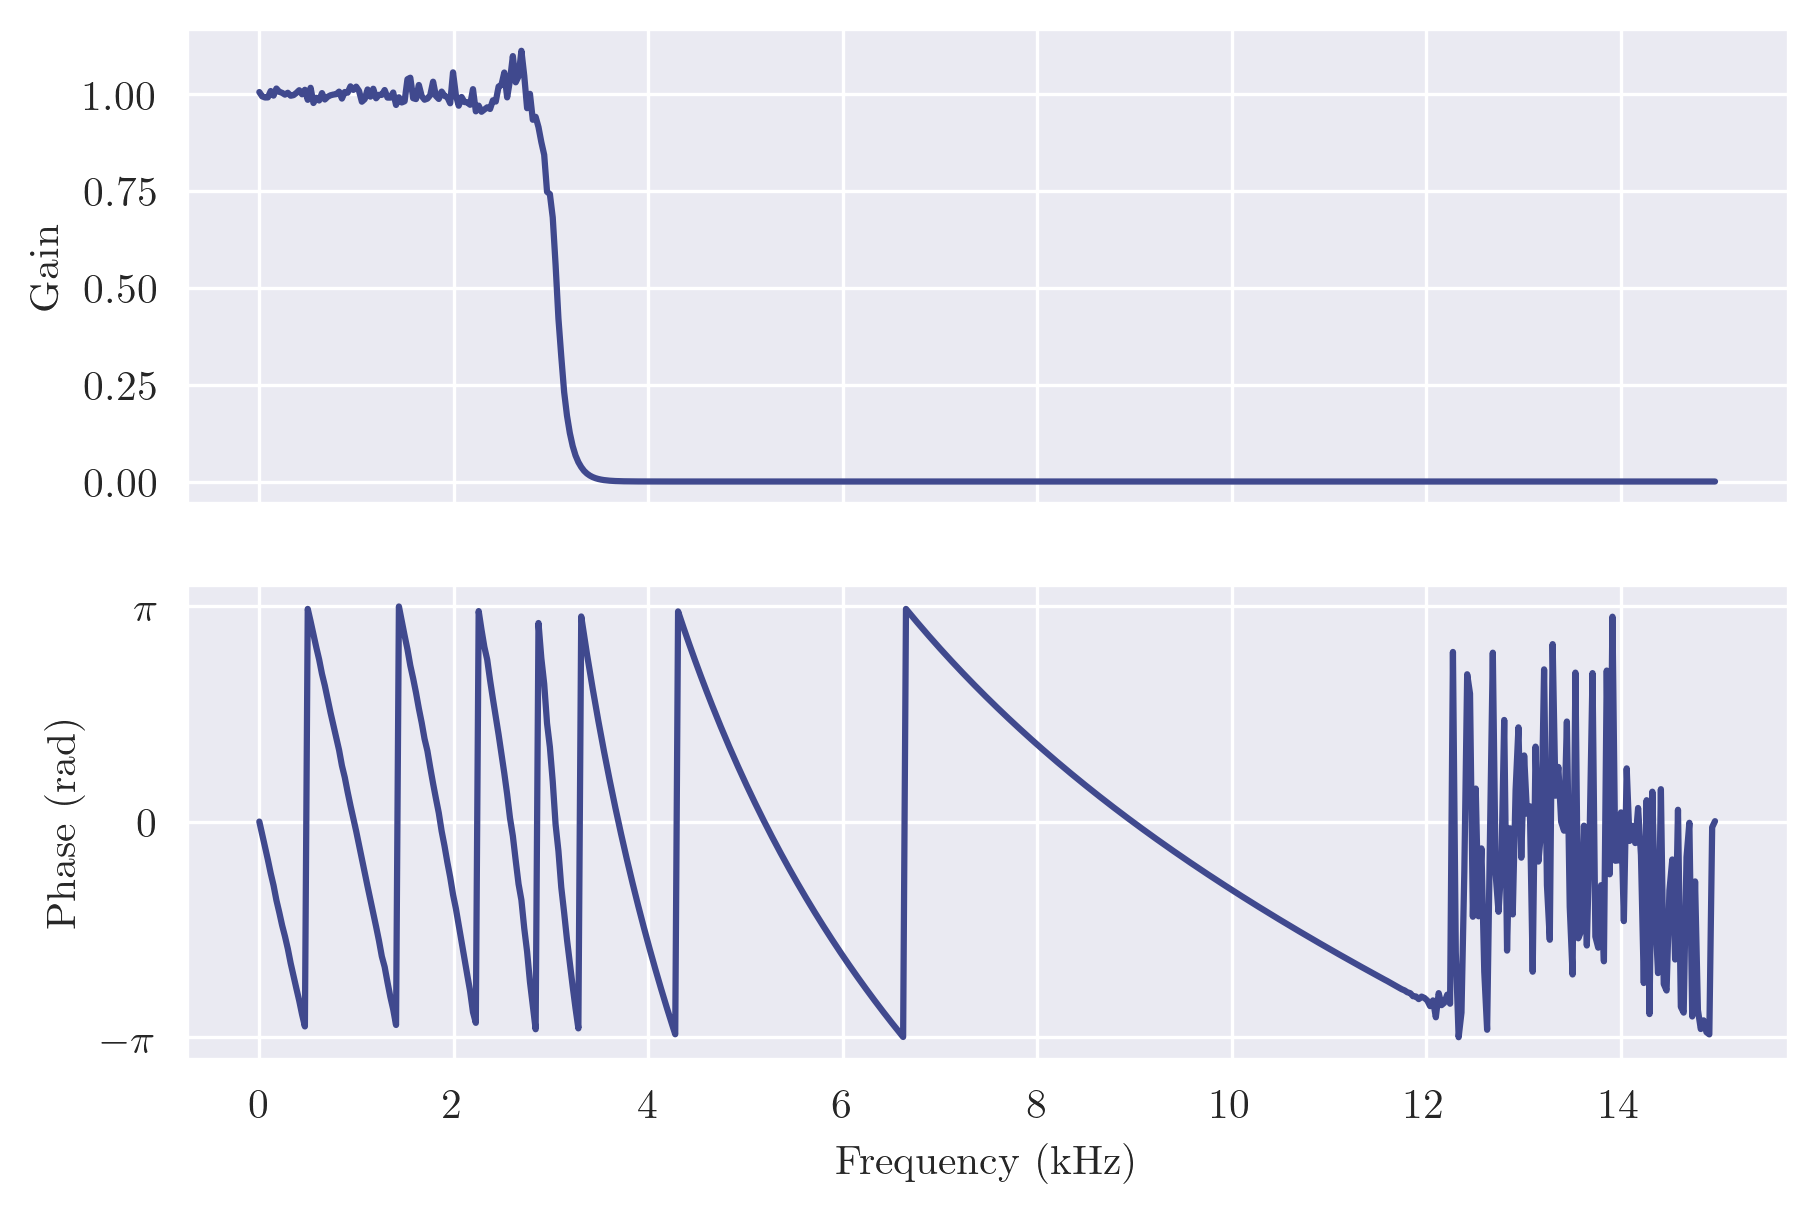
\includegraphics[width=\textwidth]{images/q8_31th_freqz.png}
    \end{subfigure}
    \hfill
    \begin{subfigure}[b]{0.25\textwidth}
        \centering
        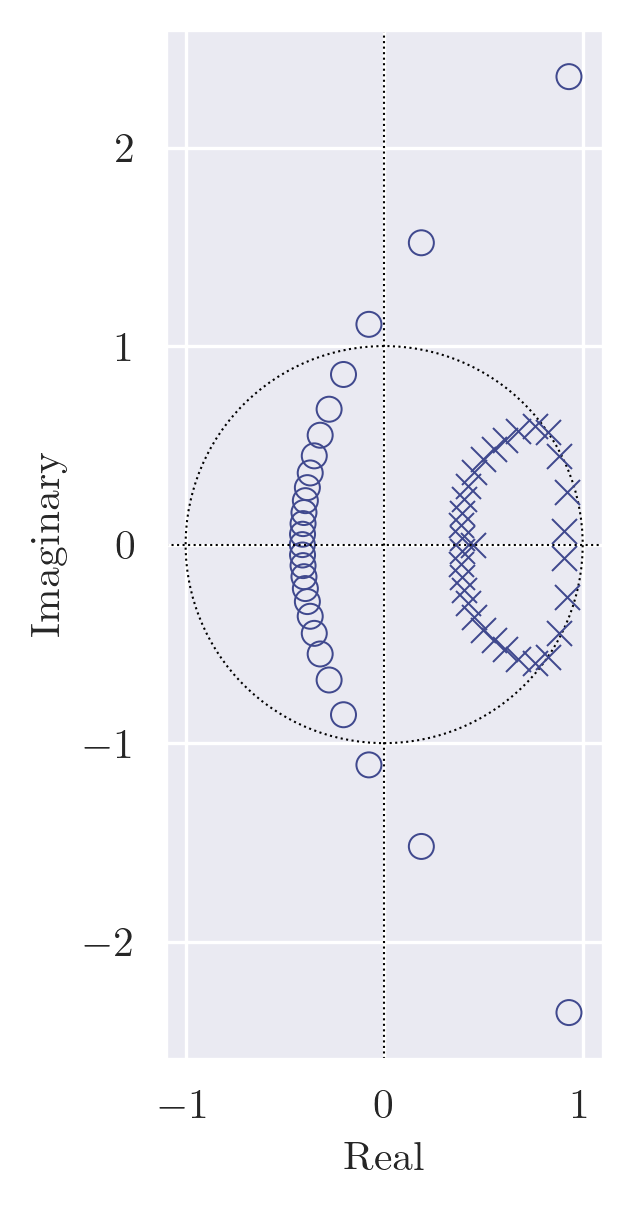
\includegraphics[width=\textwidth]{images/q8_31th_zp.png}
    \end{subfigure}
    \caption{Frequency response and pole-zero plot of 31st-order low pass Butterworth filter}
\end{figure}

\begin{figure}[!ht]
    \centering
    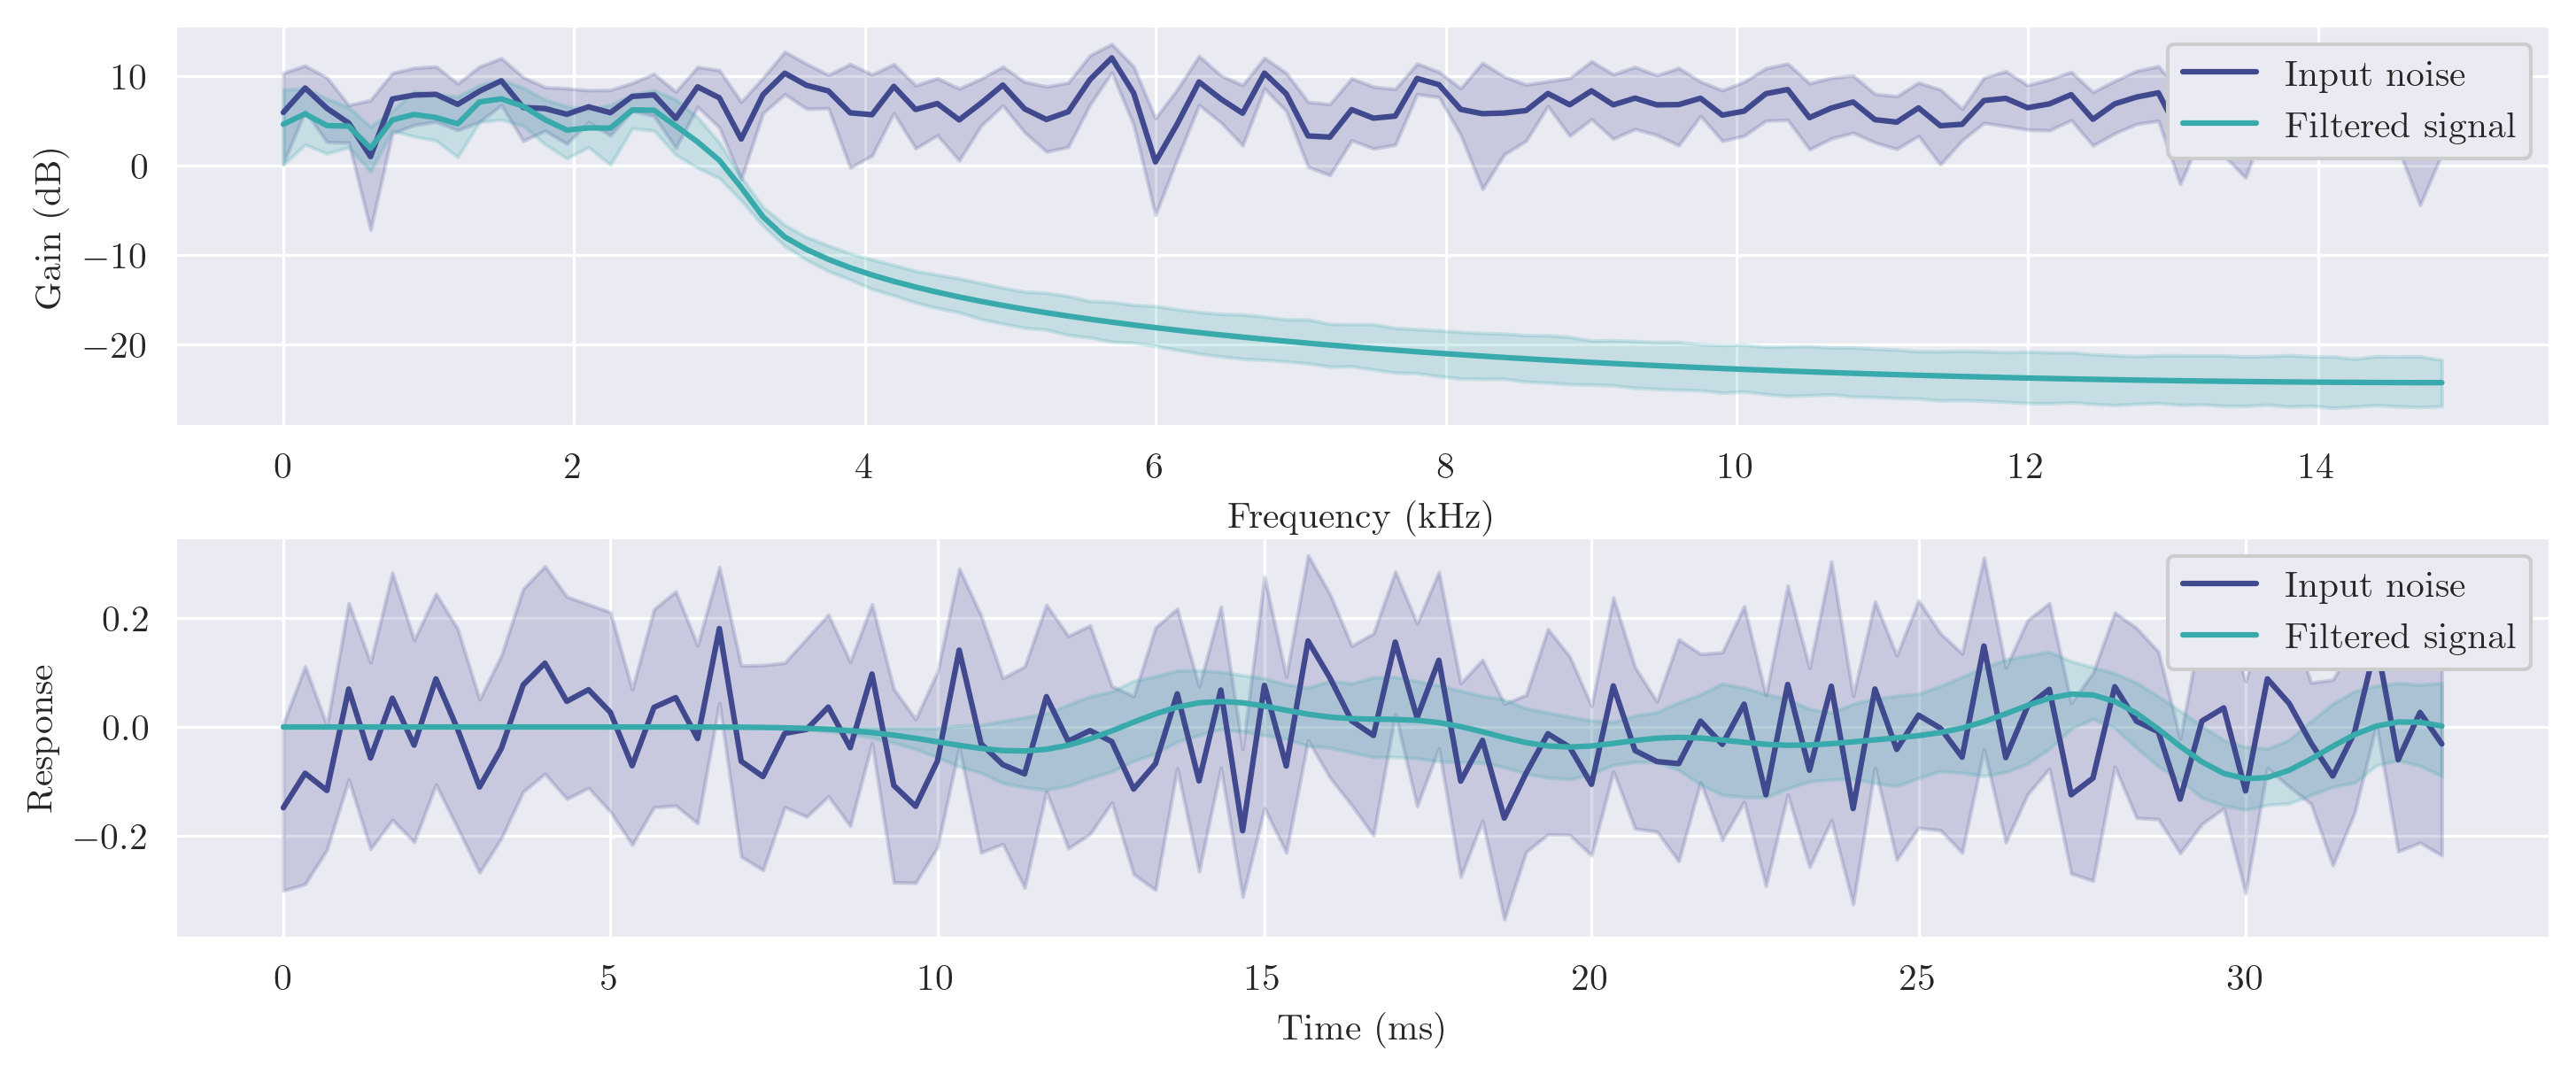
\includegraphics[width=0.99\textwidth]{images/q8_31th_stability.png}
    \caption{Original and (31st-order) filtered noise signals using unquantized coefficients}
\end{figure}

\newpage
{\Large\textbf{Filter Order: 32 (Unquantized)}}
\vspace{1em}

\begin{figure}[ht]
    \centering
    \begin{subfigure}[b]{0.73\textwidth}
        \centering
        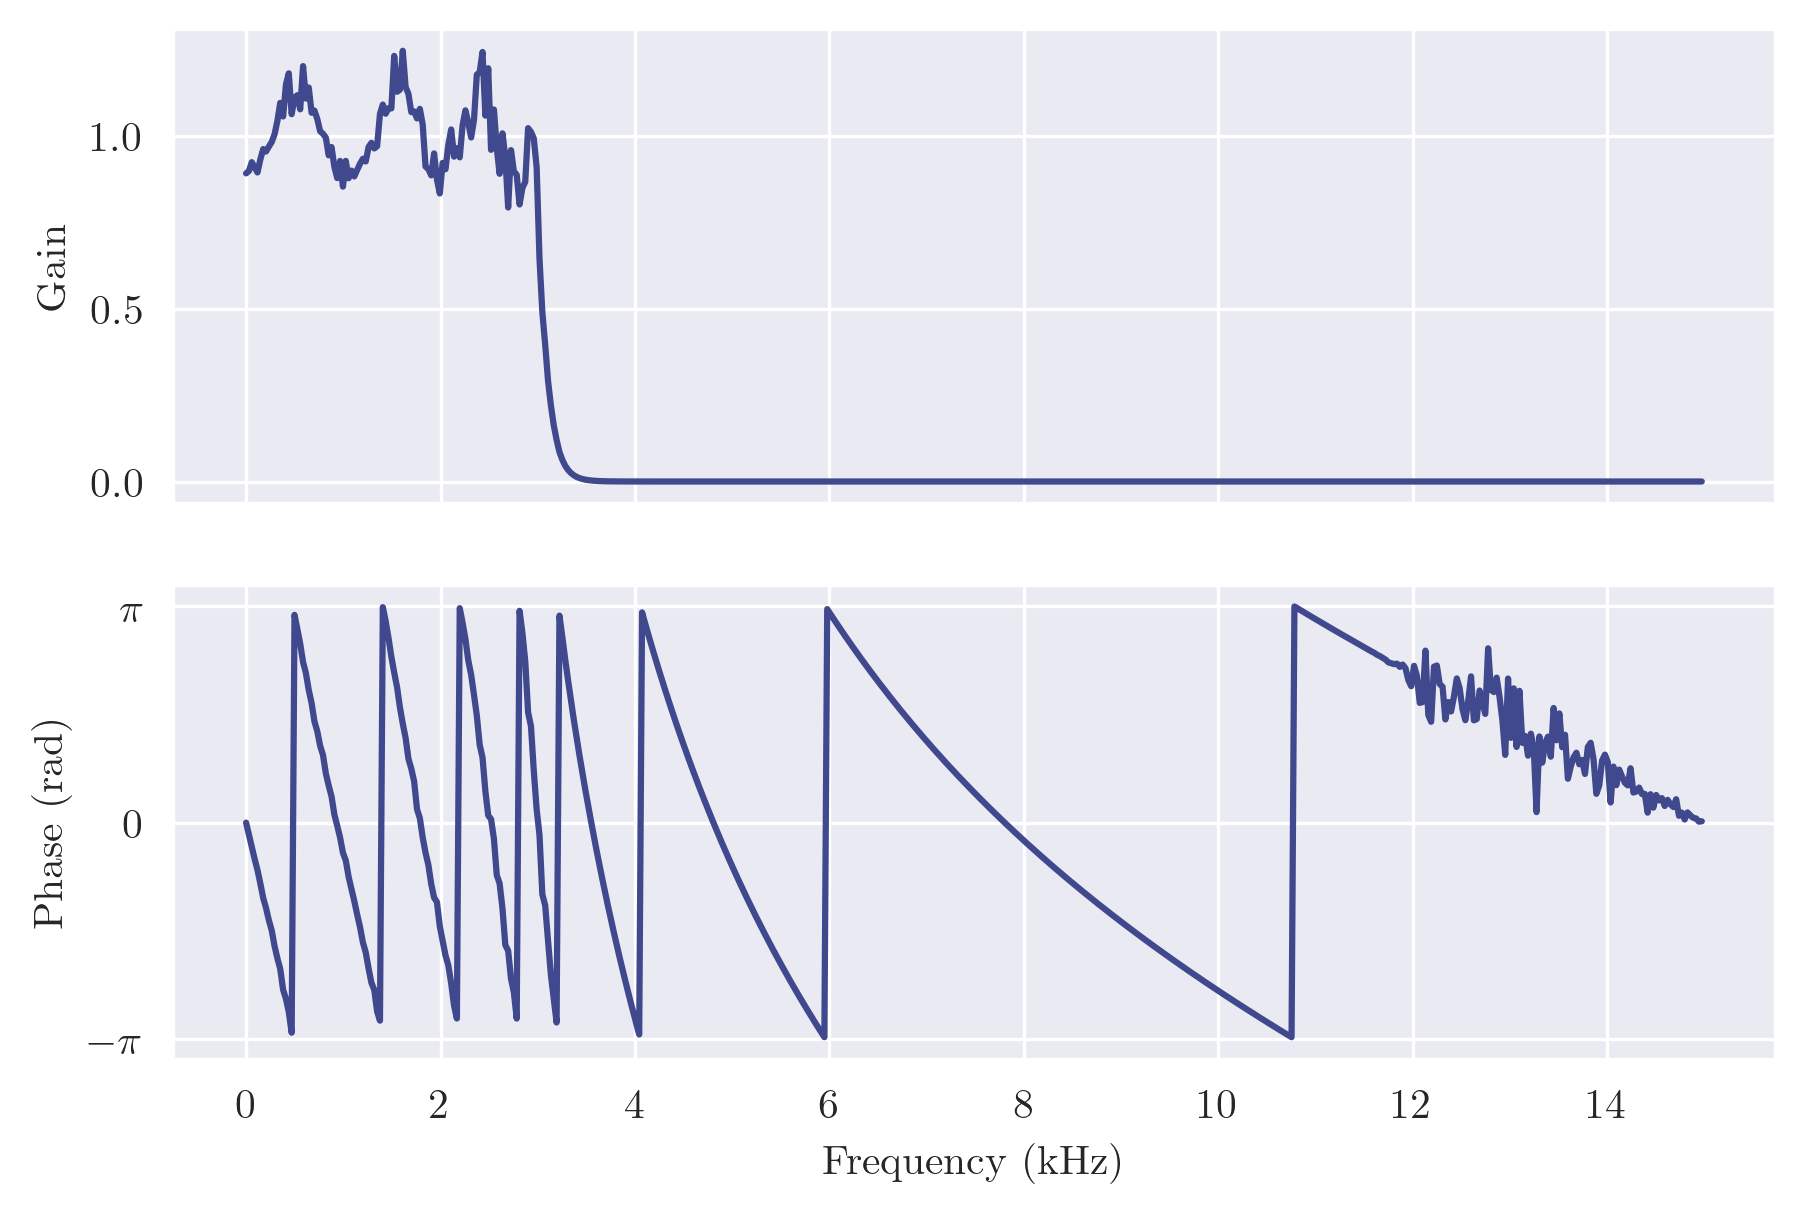
\includegraphics[width=\textwidth]{images/q8_32th_freqz.png}
    \end{subfigure}
    \hfill
    \begin{subfigure}[b]{0.25\textwidth}
        \centering
        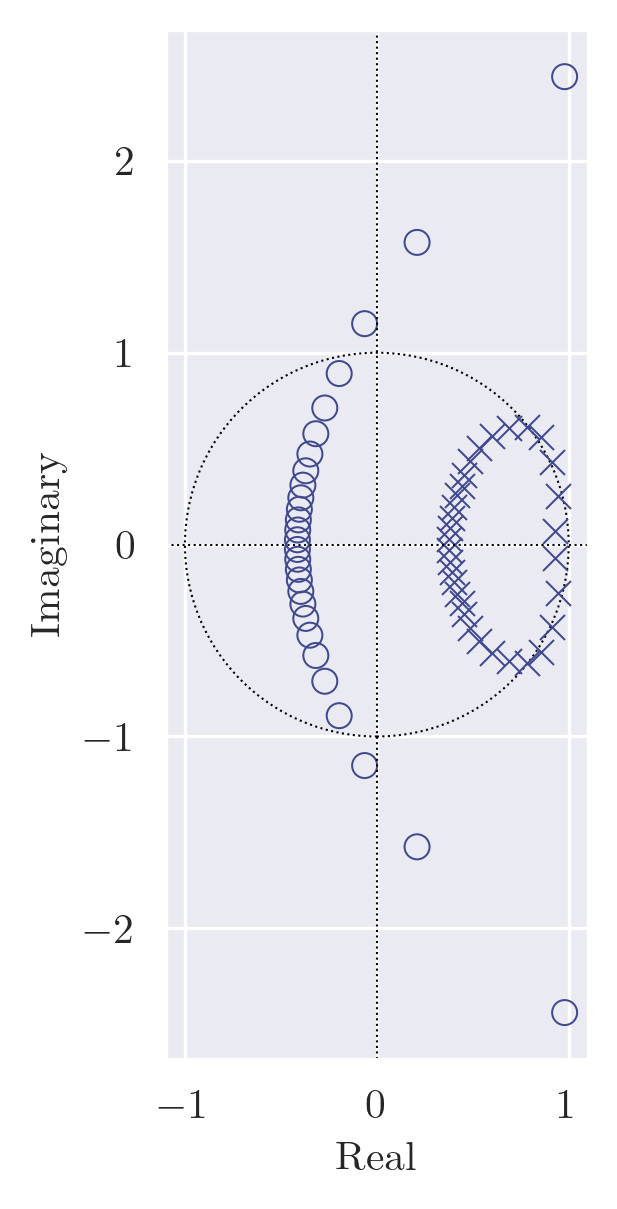
\includegraphics[width=\textwidth]{images/q8_32th_zp.png}
    \end{subfigure}
    \caption{Frequency response and pole-zero plot of 32nd-order low pass Butterworth filter}
\end{figure}

\begin{figure}[!ht]
    \centering
    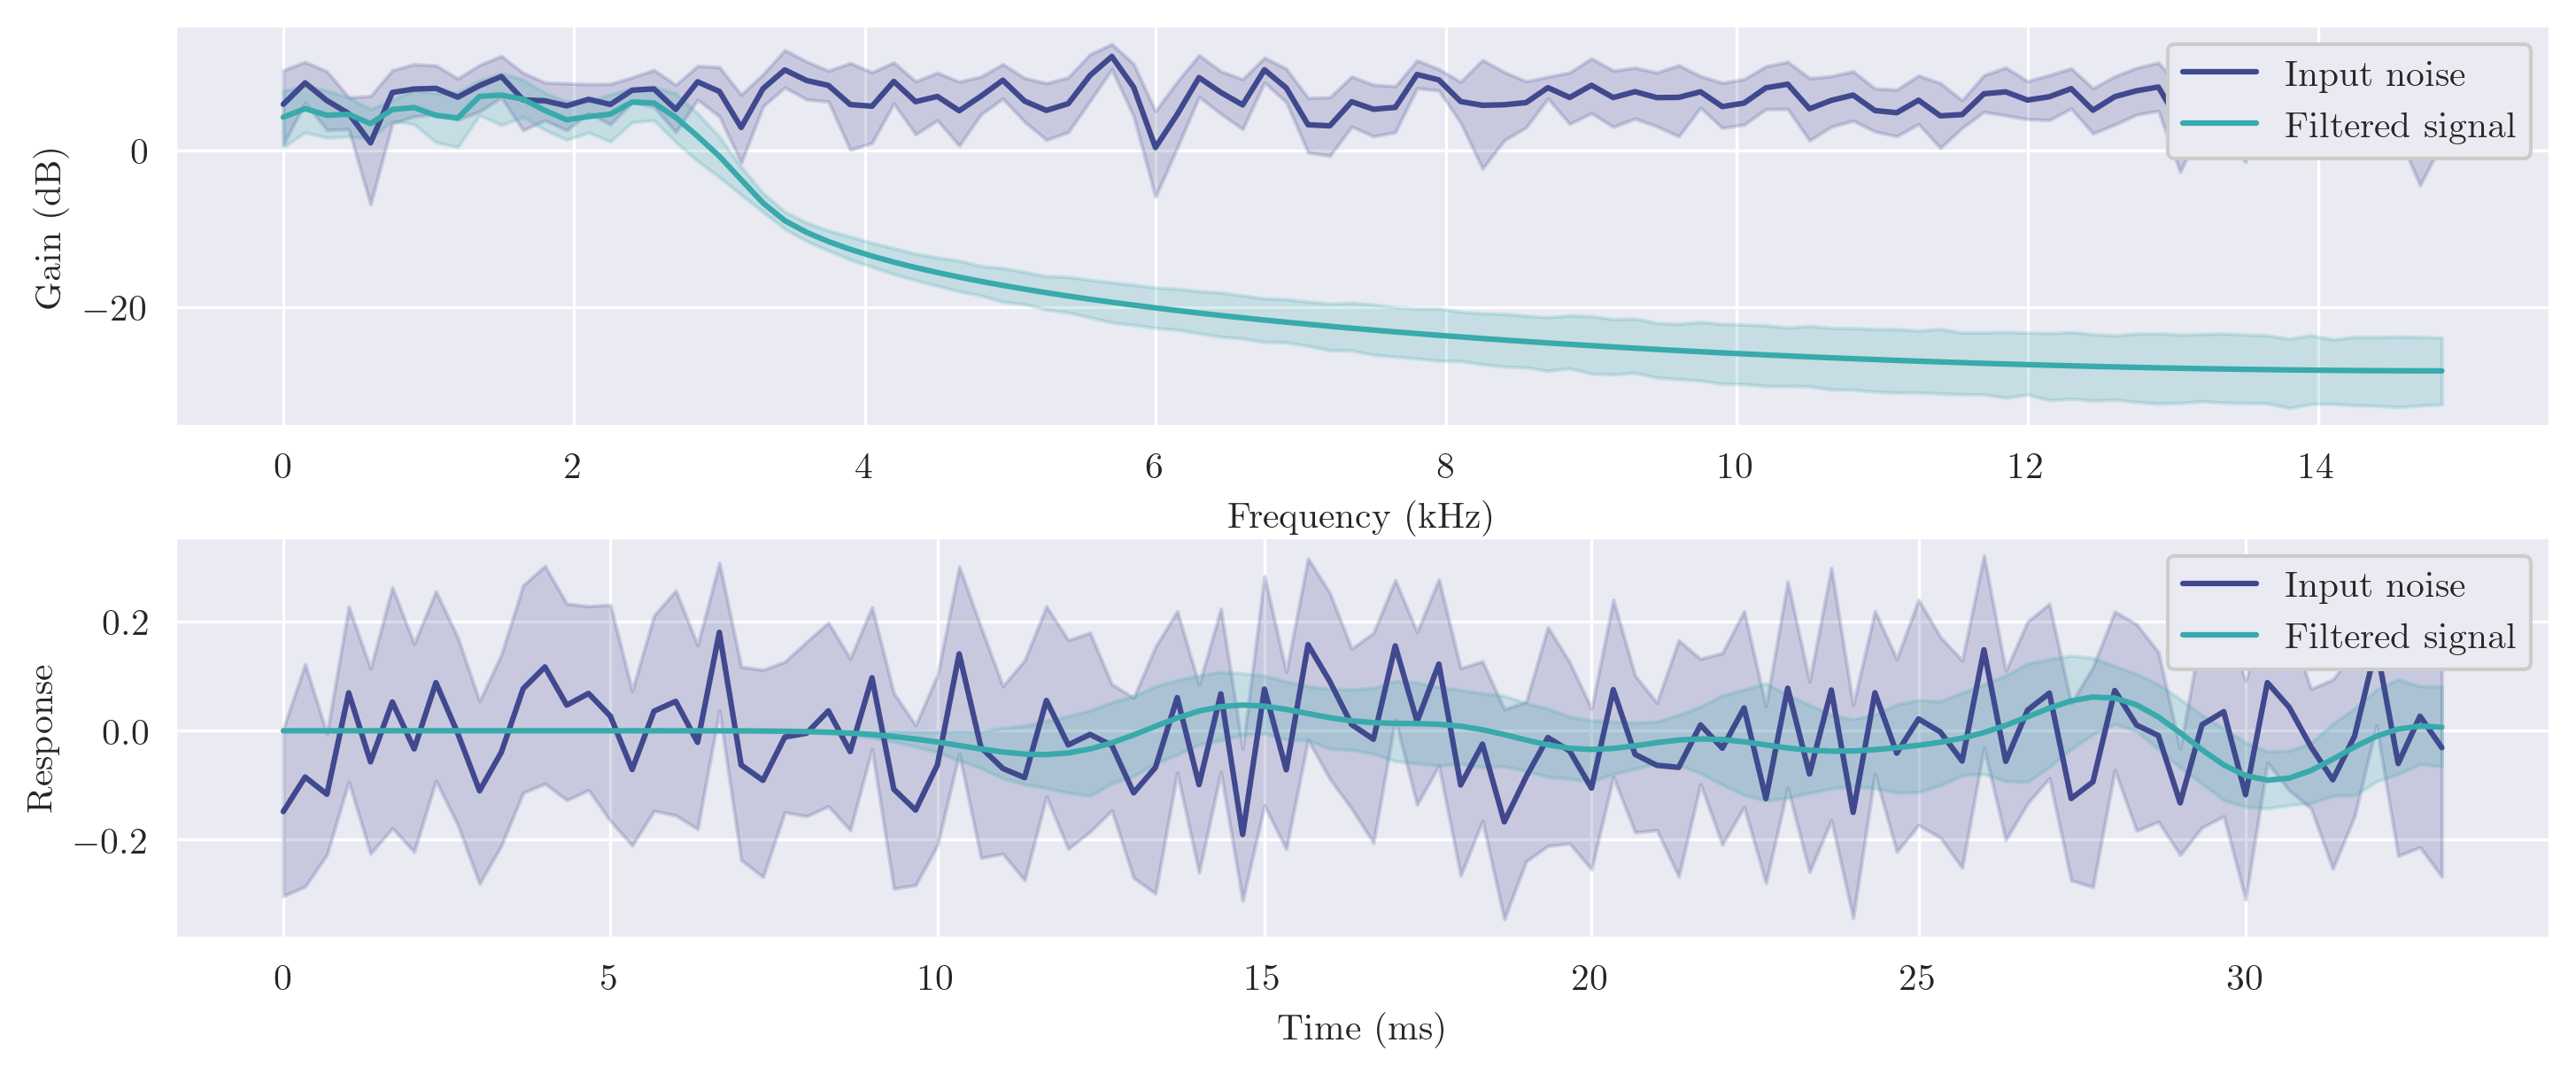
\includegraphics[width=0.99\textwidth]{images/q8_32th_stability.png}
    \caption{Original and (32nd-order) filtered noise signals using unquantized coefficients}
\end{figure}
